\documentclass[a4paper,twoside,phd]{BYUPhys}
% The BYUPhys class is for producing theses and dissertations
% in the BYU Department of Physics and Astronomy.  You can supply
% the following optional arguments in the square brackets to
% specify the thesis type:
%
%   senior  : Produces the senior thesis preliminary pages (default)
%   honors  : Produces the honors thesis preliminary pages
%   masters : Produces the masters thesis preliminary pages
%   phd     : Produces the PhD dissertation preliminary pages
%
% The default format is appropriate for printing, with blank pages
% inserted after the preliminary pages in twoside mode so you can
% send it directly to a two-sided printer. However, for ETD
% submission the blank pages need to be removed from the final output.
% The following option does this for you:
%
%   etd     : Produces a copy with no blank pages in the preliminary section.
%             Remove this option to produce a version with blank pages inserted
%             for easy double sided printing.
%
% The rest of the class options are the same as the regular book class.
% A few to remember:
%
%   oneside : Produces single sided print layout (recommended for theses less than 50 pages)
%   twoside : Produces double sided print layout (the default if you remove oneside)
%
% The BYUPhys class provides the following macros:
%
%   \makepreliminarypages : Makes the preliminary pages
%   \clearemptydoublepage : same as \cleardoublepage but doesn't put page numbers
%                           on blank intervening pages
%   \singlespace          : switch to single spaced lines
%   \doublespace          : switch to double spaced lines
%
% --------------------------- Load Packages ---------------------------------

% The graphicx package allows the inclusion of figures.  Plain LaTeX and
% pdfLaTeX handle graphics differently. The following code checks which one
% you are compiling with, and switches the graphicx package options accordingly.
\usepackage{ifpdf}
\ifpdf
  \usepackage[pdftex]{graphicx}
\else
  \usepackage[dvips]{graphicx}
\fi

%%%%%%%%%%%%%%%%%%%%%%%%%%%%%%%%%%%%%%%%%%%%%%%%%%%%%%%%%%%%%%%%%%
% Edited : Beeshanga
%
% If you need to include any code in the text use this package
% \usepackage{listings}
% It can be used to make key words bold, add colours, etc. Refer
% to http://en.wikibooks.org/wiki/LaTeX/Packages/Listings for
% more information.
%
% For theorems, propositions, proofs and assumtions use this
% package
% \usepackage{amsthm}
% For more information refer to the following website
% http://en.wikibooks.org/wiki/LaTeX/Theorems
%
%%%%%%%%%%%%%%%%%%%%%%%%%%%%%%%%%%%%%%%%%%%%%%%%%%%%%%%%%%%%%%%%%%

% The fancyhdr package allows you to easily customize the page header.
% The settings below produce a nice, well separated header.
\usepackage{fancyhdr}
  \fancyhead{}
  \fancyhead[LO]{\slshape \rightmark}
  \fancyhead[RO,LE]{\textbf{\thepage}}
  \fancyhead[RE]{\slshape \leftmark}
  \fancyfoot{}
  \pagestyle{fancy}
  \renewcommand{\chaptermark}[1]{\markboth{\chaptername \ \thechapter. #1}{}}
  \renewcommand{\sectionmark}[1]{\markright{\thesection \ #1}}


% The cite package cleans up the way citations are handled.  For example, it
% changes the citation [1,2,3,6,7,8,9,10,11] into [1-3,6-11].  If your advisor
% wants superscript citations, use the overcite package instead of the cite package.
\usepackage{cite}

% The makeidx package makes your index for you.  To make an index entry,
% go to the place in the book that should be referenced and type
%  \index{key}
% An index entry labeled "key" (or whatever you type) will then
% be included and point to the correct page.
%\usepackage{makeidx}
%\makeindex

% The url package allows for the nice typesetting of URLs.  Since URLs are often
% long with no spaces, they mess up line wrapping.  The command \url{http://www.physics.byu.edu}
% allows LaTeX to break the url across lines at appropriate places: e.g. http://www.
% physics.byu.edu.  This is helpful if you reference web pages.
\usepackage{url}
\urlstyle{rm}

% If you have a lot of equations, you might be interested in the amstex package.
% It defines a number of environments and macros that are helpful for mathematics.
% We don't do much math in this example, so we haven't used amstex here.
\usepackage{amsmath}
\usepackage{amssymb}
\usepackage{subfigure}
\usepackage{cite}
\usepackage{amsxtra}
\usepackage{amsfonts}
\usepackage{graphicx}
\usepackage[table]{xcolor}
\usepackage{longtable}
\usepackage{listings}
\usepackage{multirow} % This is package for multi-rows in tables added on 7th July 2009 by Arif
%\usepackage{setspace}

% The caption package allows us to change the formatting of figure captions.
% The commands here change to the suggested caption format: single spaced and a bold tag
\usepackage[labelfont=bf,labelsep=colon]{caption}%[2008/04/01]
 \DeclareCaptionFormat{suggested}{\singlespace#1#2#3\par\doublespace}
 \captionsetup{format=suggested}


\usepackage{array}
\usepackage{multirow}
\usepackage{verbatim}
\usepackage{enumerate}

% Defining the symbols




% The hyperref package provides automatic linking and bookmarking for the table
% of contents, index, equation references, and figure references.  It must be
% included for the BYU Physics class to make a properly functioning electronic
% thesis.  It should be the last package loaded if possible.
%
% To include a link in your pdf use \href{URL}{Text to be displayed}.  If your
% display text is the URL, you probably should use the \url{} command discussed
% above.
%
% To add a bookmark in the pdf you can use \pdfbookmark.  You can look up its usage
% in the hyperref package documentation
\usepackage[bookmarksnumbered,pdfpagelabels=true,plainpages=false,colorlinks=true,
            linkcolor=black,citecolor=red,urlcolor=blue]{hyperref}

% ------------------------- Fill in these fields for the preliminary pages ----------------------------
%
% For Senior and honors this is the year and month that you submit the thesis
% For Masters and PhD, this is your graduation date
  \Year{2018}
  \Month{November 09,}
  \Author{Abhishek Satpathy}

% If you have a long title, split it between two lines. The \TitleBottom field defines the second line
% A two line title should be an "inverted pyramid" with the top line longer than the bottom.
    \TitleTop{Framework for Interoperability and Scalability }
  \TitleBottom{of Blockchains and Token Systems} % edited Beeshanga
 \DegreeTitle{Bachelor of Engineering
 \\ Software Engineering Stream} % edited Beeshanga

% Your research advisor
 \Advisor{Supervisor: Michael Johnson}

% The department undergraduate research coordinator
%  \UgradCoord{A}

% The representative of the department who will approve your thesis (usually the chair)
%  \DepRep{B}

% Acknowledge those who helped and supported you

  \Acknowledgments{
  \vspace{-1.5cm}
    \noindent I would like to acknowledge my supervisor Prof. Michael Johnson who has always been a great help throughout my degree and not just this thesis. Michael accepted to supervise my project proposal even though it was not related to one of his areas of research. 
    \\
    \indent I would also like to acknowledge Mr. Kris Crnomarkovic who has been really helpful with long and tiring discussions about certain difficult issues that I encountered during research. Kris's involvement with my theses is really appreciated. I am also deeply grateful to my co-founder and friend Andrew for pushing me hard to finish my thesis on time and helping me with numerous suggestions and edits. Without him, I would not even be close to finishing it on time. And finally, I would like to thanks everyone at the incubator for being supportive of me while I was working long hours and for keeping a progress check on the writing.

  }


% The title of the department representative
%  \DepRepTitle{Chair}
  \Statement{
    \noindent I, Abhishek Satpathy, declare that this report, submitted as part of the requirement for the award of Bachelor of Engineering in the School of Engineering, Macquarie University, is entirely my own work unless otherwise referenced or acknowledged. This document has not been submitted for qualification or assessment at any other academic institution.
    \vspace{0.5cm}

    \noindent     Student's Name: Abhishek Satpathy

    \vspace{0.25cm}

    \noindent Student's Signature: Abhishek Satpathy

    \vspace{0.25cm}

    \noindent     Date: \today
    }

% The text of your abstract
\Abstract{
\vspace{-1.5 cm}
Blockchain technology has potential applicability in finance, supply chain management, asset tracking, and web decentralization. Scalability and interoperability are two major problems, hindering the applicability of blockchains in large-scale commercial architectures. In this thesis, we discuss the architecture of a novel framework that aims to solve the issues of scalability and interoperability of blockchains using a communication layer between multiple compatible blockchains. The communication layer has a central blockchain which is capable of supporting multiple token systems. The central blockchain is capable of transferring tokens among those multiple blockchains securely.
}



% Statement of Candidate



\fussy

\begin{document}

 % Start page counting in roman numerals
 \frontmatter

 %This command makes the formal preliminary pages.
 % You can comment it out during the drafting process if you want to save paper.

 \makepreliminarypages


%\clearemptydoublepage
\doublespace
%\include{Publications/publications}

% \clearemptydoublepage
%\include{Organization/organization}

 \clearemptydoublepage
\singlespace
 % Make the table of contents.
 \tableofcontents

\clearemptydoublepage
% Make the list of figures
\listoffigures

\clearemptydoublepage
% Make the list of tables
\listoftables

\clearemptydoublepage

% Start regular page counting at page 1
\mainmatter
%
\chapter{Introduction}
\label{chap:Introduction}
Blockchain technology has demonstrated enormous potential utility in multiple fields including ``Internet of things", governance, finance, asset-tracking, and web decentralization. However, the widespread adoption and use of blockchains into commercial applications yet to be demonstrated.\cite{GavinWood2018POLKADOT:FRAMEWORK}
 Scalability and interoperability are major problems, hindering the production-grade adoption of blockchains into these different fields of application.\cite{TheZilliqaTeam2017TheWhitepaper} Blockchain systems currently are lagging behind due to extremely low transaction throughput which makes their use impractical in real-world use cases\cite{GavinWood2018POLKADOT:FRAMEWORK}. Available blockchain implementations are practically limited to approximately 30 transactions per second \cite{GavinWood2018POLKADOT:FRAMEWORK}. This issue of limited transaction throughput arises from the current synchronous consensus mechanisms which require a wide time margin to ensure the safety of transactions \cite{GavinWood2018POLKADOT:FRAMEWORK}. The demand for higher transaction throughput is increasing with the growing user base\cite{Croman2016OnBlockchains}. One way of addressing this scalability problem is facilitating intercommunication among smart contracts on multiple separate blockchains\cite{Kwon2018ALedgers}. This intercommunication framework inherently solves the problem of interoperability along with scalability. In this thesis, we lay out the design, testing, and implementations specifications of such a framework.
 
\section{Project Goal}
The goal of this project is to lay out the design, testing, and design specifications of a layer two blockchain solution that facilitates higher transaction throughput and interoperability among multiple blockchain systems. Layer two is defined as a system that is built on top of a layer one blockchain system like Ethereum or bitcoin and therefore relies on the layer one chain for security \cite{MichaelJCaseyLayerCoinDesk}. Layer two solutions are built without requiring any breakthrough modifications to the existing layer one architecture\cite{MichaelJCaseyLayerCoinDesk}. The project is specifically going to focus on a protocol that is built on top of Ethereum as the foundation layer one blockchain. The biggest challenge for the implementation of this project is ensuring that the layer two solution is at least as secure as the existing foundation that it is built upon. The protocol has to balance between keeping a high transaction throughput and maintaining a high level of decentralization. Decentralization and transaction throughput can easily get inversely intertwined in a decentralized system architecture and therefore precaution needs to be taken while designing the system to reduce centralization.
\\
\\ One of the other goals of the project will also be to lay out the modifications to the existing foundation system that would allow the integration of the layer two system to the foundation architecture. The project does not aim to create a completely new blockchain architecture.
\section{Project Planning}
The project planning was done over the last six months during the course of ENGG 460. There have been a lot of changes the initial plan that was developed during ENGG 460. The biggest change, however, has been to the scope, deliverables, and timeline of the project. These changes are discussed below in their respective sections.

\subsection{Scope}
The project scope has remained very similar to the scope that was described in the initial project plan. The scope is to deliver a protocol for intercommunication and interoperability of smart contracts. The scope in the initial project plan might have indicated that the scope includes the delivery of a prototype of such a blockchain architecture; however, the new scope of the project includes only the system requirements, design and testing specifications of the protocol. 
\subsection{Deliverables}
The initial project plan specified two deliverables. One of the deliverables for the project was a suite of smart contracts on different Ethereum blockchains such that those smart contracts can send messages and transactions among themselves. The other deliverable in the initial project plan was a react-native app that would be able to demonstrate the functionality of the smart contracts. There has been a change in the deliverables for the project over the course of the last six weeks of progressing through the development. 
\\

The new deliverable for the project is a framework for intercommunication and the interoperability of multiple blockchains. The deliverable includes system requirements, system testing, and implementation specifications. However, any working prototype of the protocol is not a hard deliverable of the project.
\subsection{Timeline}
There have been significant changes to the timeline of the project as it has progressed. The reason for these changes is the change in the deliverables for the project. The deadline for the project was assumed to be mid-December in the previous project plan; the new deadline is the 9th of November which is a hard deadline. Moreover, a lot of variables and deliverables had unknown components with estimated timeframes. The timeline has a become firmer with most of the variables becoming clearer. The new GANTT chart with the updated timeline for the project is given in appendix c.
\section{Project Background}
Prior to starting in on blockchain systems, one needs to be familiar with supporting technologies that support and facilitate the working of blockchains. 
\subsection{Cryptographic Hash Function}
A cryptographic hash function is a one-way mathematical construct that takes a data input of arbitrary length and outputs arbitrary data of a fixed length \cite{PreneelCRYPTOGRAPHICOVERVIEW}. The primary use of hashing in blockchains is maintaining the integrity of messages\cite{2018WhatAcademy}. Hashes are used in a blockchain to ensure the integrity of the data stored in each block. The data or the list of transactions in a block is hashed and the hash is appended to the next block, this ensures the integrity of the data because if even a single bit of the data is manipulated then the new hash of the block is completely different\cite{PreneelCRYPTOGRAPHICOVERVIEW}. The hash function used in the protocol described in this paper is Keccac-512 which is a variation of the SHA-512 hashing algorithm\cite{Bertoni2012KeccakOverview}. 
\subsection{Public Key Cryptography}
Public Key Cryptography is one of the core technologies used in a blockchain system. The accounts on a blockchain are a hashed version of the public key of the user\cite{Wood2018ETHEREUM:LEDGER}. The accounts can be viewed using the public key of the account, but in order to use or transfer funds held in the account, the private key is required\cite{ButerinAPLATFORM}.
\subsection{Consensus}
Consensus is a mechanism which ensures that every node on the blockchain network has the same exact copy of the data \cite{ChrisHammerschmidt2017ConsensusMedium}. A consensus mechanism synchronizes data across all nodes as and when those nodes connect to the network\cite{TendermintTeam2018WhatDocumentation}. Consensus also works as a fault tolerance mechanism which is essential in any distributed computing setup such as a distributed ledger to avoid corrupt nodes\cite{ConsensusInvestopedia}. Proof of work is by far the most popular consensus mechanism used in mainstream public blockchains \cite{RayahMajor2018Proof-of-StakePOW}. It is ultimately a variation of the popular Practical Byzantine Fault tolerance algorithm \cite{RayahMajor2018Proof-of-StakePOW}.
\subsection{State Transition Machine}
The state of a blockchain is the mapping between the account addresses and the state of the account in terms of the transaction history\cite{Wood2018ETHEREUM:LEDGER}. Every transaction on the blockchain is a manipulation of the state. The blockchain itself acts as a state transition machine which facilitates transactions by allowing the valid ones to manipulate the state\cite{ButerinAPLATFORM}.
\subsection{Clients}
A client of the blockchain is the end-user software that ensures the blockchain synchronisation, generates and stores private keys, and facilitates transactions on behalf of the private key \cite{2018ClientsWiki}. Clients live on user hardware which acts as an interface between the user's device and the blockchain network\cite{ButerinAPLATFORM}.
\subsection{Transactions}
A transaction is the transfer of a signed data package on the blockchain which manipulates the state of the ledger\cite{ButerinAPLATFORM}. It is a record of a valid computational activity that has taken place. Any information that is stored and can be retrieved is the result of a transaction. EVM transactions involve a transfer of value as the transactions themselves have a cost attached to them\cite{ButerinAPLATFORM}. 
\subsection{Smart Contracts}
Smart Contracts are agents that facilitate the negotiation of a transaction on the blockchain without the use of another third party agent\cite{ButerinAPLATFORM}. Smart contracts are the only entry point to the state of the blockchain and therefore the only party that can modify the data layer on the ledger\cite{ButerinAPLATFORM}.

\chapter{Background and Related Work}
This chapter reviews the existing literature and work done in the area of increasing blockchain transaction throughput by facilitating interoperability of blockchains. The most important thing to note is that there is a serious lack of qualitative academic literature in the field as the research in the field is quite new and hasn't percolated into academia yet. Therefore, most of the available literature is from research work done by blockchain startups and the available whitepapers. The language in those whitepapers is often not very academic. Therefore, one of the most important tasks in this chapter would be to interpret the relevant whitepapers critically.
\section{Ethereum}
Ethereum is a decentralised value transfer system made possible using a cryptographically secure, transaction-based state machine. Which is a blockchain or a distributed ledger in simple terms\cite{ButerinAPLATFORM}. Ethereum was first developed by Vitalik Buterin in late November 2013\cite{ButerinAPLATFORM}. It was a complete rewrite of the bitcoin system with the addition of a Turing complete virtual machine and smart contract execution capability\cite{ButerinAPLATFORM}. In Ethereum's state transition machine, the final state also referred to as the canonical state is a result of a consensus mechanism using a simplified version of the GHOST protocol\cite{Wood2018ETHEREUM:LEDGER}.

\subsection{Blocks, State and Transactions}
\subsubsection{Blocks}
The block in Ethereum is a collection of transactions bunched together as a set\cite{ButerinAPLATFORM}. The block has three parts, a block header, the transactions, and the ommers, a collection of related block headers\cite{Wood2018ETHEREUM:LEDGER}. The block header contains the following pieces of information as stated in the Ethereum yellowpaper\cite{Wood2018ETHEREUM:LEDGER}
\begin{description}
\item[$\bullet$ parentHash:] a Keccak 256-bit hash of the previous block's header
\item[$\bullet$ ommersHash:] a Keccak 256-bit hash of the ommers list or the list of blocks which have the same parent block as the current block
\item[$\bullet$ beneficiary:] the 160-bit address of the account to which all the gas fee has to be transferred
\item[$\bullet$ stateRoot:] a Keccak 256-bit hash of the root node of the state trie
\item[$\bullet$ transactionsRoot:] a Keccak 256-bit hash of the root node of the trie containing all the transactions in the current block
\item[$\bullet$ receiptsRoot:] a Keccak 256-bit hash of the trie containing the reciepts of all the transactions in the current block
\item[$\bullet$ logsBloom:] bloom filter composed of index-able log entries for transaction receipts
\item[$\bullet$ difficulty:] a number corresponding to the difficulty level of the block
\item[$\bullet$ number:] a scalar value corresponding to the number of ancestor blocks of the current block. The genesis block does not have an ancestor block and hence, it is conventionally assigned a number 0.
\item[$\bullet$ gasLimit:] a scalar value equal to the maximum limit of gas expenditure of the block
\item[$\bullet$ gasUsed:] a scalar value equal to the total gas used in transactions in the block
\item[$\bullet$ timeStamp:] a reasonable output of the Unix time at the block's inception
\item[$\bullet$ extraData:] arbitrary byte array containing block metadata
\item[$\bullet$ mixhash:] a 256-bit hash which together with the nonce proves that a sufficient amount of computation has been carried out on this block
\item[$\bullet$ nonce:] a 64-bit hash which together with the mix-hash proves that a sufficient amount of computation has been done on this block
\end{description}
\subsubsection{World State}
The world state is a mapping between account addresses which are 160 bit hashed versions of the public keys and account states\cite{Wood2018ETHEREUM:LEDGER}. This mapping is stored in a data structure called a Merkle Patricia tree. The account states comprise of the following fields as stated in the Ethereum Yellowpaper\cite{Wood2018ETHEREUM:LEDGER}:
\begin{description}
\item[$\bullet$ nonce:] it is a value that is equal to the number of transactions sent from the account
\item[$\bullet$ balance:] a value equal to the number of Wei owned by the address
\item[$\bullet$ storageRoot:] a 256-bit hash of the root node of the Merkle Patricia tree that contains the storage data of the account
\item[$\bullet$ codeHash:] the hash of the Ethereum Virtual Machine (EVM) code of the account, which gets executed in case of transactions
\end{description}
\subsubsection{Transactions}
A transaction is formally a single cryptographically signed instruction executed by an external party\cite{ButerinAPLATFORM}. There are two types of transactions in Ethereum: the first type results in a message call between actors and the second type results in the creation of new accounts\cite{Wood2018ETHEREUM:LEDGER}. A transaction primarily has the following fields as stated in the Ethereum Yellowpaper\cite{Wood2018ETHEREUM:LEDGER}:
\begin{description}
\item[$\bullet$ nonce:] a value equal to the number of transactions sent by the sender
\item[$\bullet$ gasPrice:] number of wei to be paid for each unit of gas. Gas is a computational unit in the EVM which is discussed in a later section.
\item[$\bullet$ gasLimit:] maximum amount of gas that should be utilised for executing this transaction
\item[$\bullet$ to:] a 160-bit address of the message call's recipient 
\item[$\bullet$ value:] number of wei to be transferred to the message call's recipient
\end{description}
A contract creation account contains the following additional fields\cite{Wood2018ETHEREUM:LEDGER}:
\begin{description}
\item[$\bullet$ nonce:] infinite size byte array containing the EVM code for account initialisation
\item[$\bullet$ data:] infinite size byte array containing the input data of the message call
\end{description}
\begin{description}
\item[]
\end{description}
\subsection{Gas and Transaction Execution}
Gas and transactions are the core of the Ethereum computation engine. Transactions form the basis for all the computation and Gas forms the basis of all payment calculation in Ethereum\cite{ButerinAPLATFORM}.
\subsubsection{Gas}
Gas is defined as any programmable computation in Ethereum\cite{ButerinAPLATFORM}. The EVM is a Turing complete computation engine and it is absolutely essential to limit the possibility of denial-of-service attacks in a public computation engine\cite{ButerinAPLATFORM}. Gas costs Ether to execute and therefore prevents denial-of-service as no Ethereum account is likely to have an infinite amount of Ether\cite{ButerinAPLATFORM}. Every transaction has a Gas price which is the amount of ether paid per Gas or computational step\cite{ButerinAPLATFORM}. Miners will usually preferably select a transaction which has the highest gas price.
\subsubsection{Sub-state}
A valid transaction in Ethereum is defined as a transaction which\cite{Wood2018ETHEREUM:LEDGER}:
\begin{description}
\item [$\bullet$ is a well formed Recursive Length Prefix (RLP);]
\item [$\bullet$ has a valid signature;]
\item [$\bullet$ has a valid nonce;]
\item [$\bullet$ has a gas limit which is not less than the intrinsic Gas;]
\item [$\bullet$ has a sender whose account balance is greater than the Gas cost]
\end{description}

A transaction is also the most complex part of the EVM as it involves the state transition mechanism\cite{Wood2018ETHEREUM:LEDGER}. The virtual machine gets in transition state during the execution of the transaction, called the sub-state\cite{Wood2018ETHEREUM:LEDGER}. The sub-state creates a set of temporary accounts needed to complete the transaction, called the suicide set\cite{Wood2018ETHEREUM:LEDGER}.

The ethereum state transition function is defined as follows\cite{Wood2018ETHEREUM:LEDGER}: \[\sigma' = \upsilon(\sigma, T)\]
where $\sigma$ is the state and $\Upsilon$ is the state transition function.

\subsection{Canonicalisation}
Canonicalisation is defined as a process when the algorithm takes as input a document that has more than one possible representation and always transforms it into a canonical or consistent form\cite{2017Merkle2017}. Canonicalisation is a very important process in any blockchain architecture such as Ethereum. This ensures that all the nodes are synchronised and, therefore, are referring to the same state\cite{2017Merkle2017}. Proof-of-Work is the way by which Ethereum achieves a canonical state\cite{GavinWood2018POLKADOT:FRAMEWORK}. Canonicalisation and Consensus are closely related processes. The difference is that canonicalisation is standardisation of the multiple versions of the data and consensus is ensuring all the nodes have the same data.
\subsection{Message Call}
Message calls are defined as transactions between two or more smart contracts\cite{ButerinAPLATFORM}. The only difference from that of a transaction is that, transactions are message calls originated by an externally owned account\cite{Wood2018ETHEREUM:LEDGER}. Executing a message call requires multiple parameters. Those parameters are: sender(s), transaction originator (o), recipient (r), the account whose code is to be executed (c), available gas (g), value (v), the gas price (p), and an arbitrary length byte array which contains the input of the message call and the present depth of the message-call/contract-creation stack (e)\cite{Wood2018ETHEREUM:LEDGER}.
\\ 
\\ 
The message calls that are initiated due to VM-code execution use the following scheme\cite{Wood2018ETHEREUM:LEDGER}:
\[(\sigma', g', A, o)\equiv \Theta(\sigma, s, o, r, c, g, p, v, \Tilde{v}, d, e)\]
\\
\\
Ethereum is the most essential part of the literature review as most of the system design elements were directly or indirectly derived from variations of the design of the Ethereum system. 
\section{Cosmos}
Cosmos is a platform which facilitates the interoperability of multiple parallel blockchains while retaining the inherent security features of blockchains\cite{Kwon2018ALedgers}. One of the problems faced by interoperable multi-chain frameworks is their vulnerability to an attack if a majority of the hashing ability is not merge-mined with the central parent chain\cite{Kwon2018ALedgers}. Cosmos addresses this issue by having multiple independent blockchains which are called zones in Cosmos\cite{Kwon2018ALedgers}. The central or the parent chain is called the Cosmos hub\cite{Kwon2018ALedgers}. The zones utilise something called a Tendermint Core, which is a Practical Byzantine Fault Tolerant (PBFT) consensus engine\cite{TendermintTeam2018WhatDocumentation}. The system described in this paper uses Tendermint and it will be discussed in a later section.

The main currency on the Cosmos hub is a multi-asset proof-of-stake token\cite{Kwon2018ALedgers}. The hub and zones facilitate the intercommunication between the hub and the zones using a protocol called the inter-blockchain communication protocol, which works on a virtual UDP layer for blockchains.\cite{Kwon2018ALedgers}

\subsection{Consensus}
Cosmos uses a partially synchronous Byzantine Fault Tolerant (BFT) consensus algorithm called Tendermint\cite{Kwon2018ALedgers}. It uses optimal Byzantine Fault Tolerance with a majority of greater than 2/3 of the total voting power\cite{Kwon2018ALedgers}. Hence, more than a third of the total voting power has to be Byzantine to cause a violation of safety\cite{Kwon2018ALedgers}. As a result, when a violation occurs, it can be detected by the system by comparing conflicting blocks. And since Cosmos combined with Tendermint is a permissioned system, it is much easier to detect Byzantine nodes\cite{Kwon2018ALedgers}.

\subsection{The Hub and Zones}
The Hub and different zones in Cosmos are connected using a protocol called Inter-blockchain communication (IBC) protocol\cite{Kwon2018ALedgers}. The block commits in the zones are constantly posted on the hub, allowing the hub to keep track of the world state and also the state of the zones\cite{Kwon2018ALedgers}. The zones communicate among each other using the IBC protocol, by sending Merkle-proofs of transactions \cite{Kwon2018ALedgers}.
\subsubsection{The Hub}
The Cosmos hub is the central blockchain in the system which hosts a distributed ledger that supports multiple tokens\cite{Kwon2018ALedgers}. These coins are moved from one zone to another using a special packet in IBC called a coin packet\cite{Kwon2018ALedgers}. The hub is accountable for counting the total amount of coins in each zone. The hub is the central ledger responsible for the entire network of the zones and therefore, is a single point of failure. The security of the hub is of paramount importance. It is secured by a global set of validators which are all permissioned nodes\cite{Kwon2018ALedgers}.
\subsubsection{The Zones}
The Zones exchange information among each other via the hub using the IBC\cite{Kwon2018ALedgers}. A zone is a multi-asset, multi-signature account\cite{Kwon2018ALedgers}. The hub ensures that the zones cannot transfer more tokens than it has been assigned. The hub does not verify the authenticity of the zones and therefore it should within the senders' discretion to send tokens across zones\cite{Kwon2018ALedgers}. 
\subsection{Inter-blockchain Communication (IBC)}
The Inter-blockchain communication (IBC) works by moving packets of data from one zone to another via the hub, by posting Merkle-proofs\cite{Kwon2018ALedgers}. The proof is evidence that the sending chain published a packet which was meant for the receiving chain\cite{Kwon2018ALedgers}. 
\\
\\
The IBC is the most important component of the Cosmos literature. IBC is mentioned here because a lot of inspiration for communication between different blockchains, which have been mentioned in later chapters actually come from the IBC protocol. As shown in the diagram below, the IBC has two different types of transactions; namely, IBCBlockCommitTx transaction and an IBCPacketTx transaction\cite{Kwon2018ALedgers}. The IBCBlockCommitTx allows a zone to prove to any observer zone that its most recent block hash exists\cite{Kwon2018ALedgers}. The IBCPacketTx allows a zone to prove to any observer that a published packet was indeed sent by the sender\cite{Kwon2018ALedgers}. The separation of the two different types of transactions allows the sender and receiver zones to have independent control over their block commits, respectively. The IBCBlockCommit interaction diagram which shows the two types of transactions has been shown in figure \ref{fig:1}.
\begin{figure}
  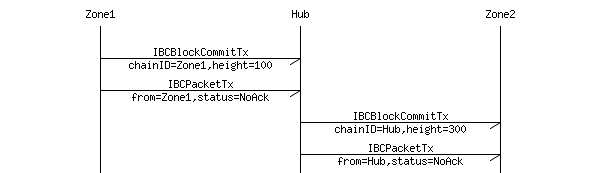
\includegraphics[width=\linewidth]{ibc_transactions.png}
  \caption{IBCBlockCommit Transaction interaction diagram\cite{Kwon2018ALedgers}.}
  \label{fig:1}
\end{figure}

\section{Zilliqa}
Zilliqa is another blockchain solution which aims to solve the problem of scalability by using blockchain sharding \cite{TheZilliqaTeam2017TheWhitepaper}. It divides the mining network into smaller shards, each capable of processing transactions in parallel\cite{TheZilliqaTeam2017TheWhitepaper}. It also has a smart contract execution environment or a virtual machine and a special contract language which implements data-flow programming\cite{TheZilliqaTeam2017TheWhitepaper}. This allows the parallel processing of the programs as soon as all the inputs are available. The entire system in Zilliqa is divided into six layers\cite{TheZilliqaTeam2017TheWhitepaper}. This layering system is good for maintenance and abstraction of different parts of the system. The layers are explained in more detail in the sections below\cite{TheZilliqaTeam2017TheWhitepaper}:

\subsection{Cryptographic Layer}
Zilliqa's cryptographic layer uses elliptic curve cryptography for digital signatures and a memory hard hash function for proof-of-work (PoW)\cite{TheZilliqaTeam2017TheWhitepaper}. The hash function used in Ziliqa is ethash, which is the hash function used in Ethereum\cite{TheZilliqaTeam2017TheWhitepaper}. Ethhash is based on Keccak, which is memory hard meaning that Application specific integrated circuits (ASIC) will not be able to generate the hashes\cite{VitalikButerin2018quotVitalikEthereum}. 
\subsubsection{EC-Schnorr Signature}
Zilliqa uses digital signatures based on the EC-Schnorr algorithm instantiated with the secp256k1 elliptic curve\cite{TheZilliqaTeam2017TheWhitepaper}. According to Zilliqa, EC-Schnorr has a few benefits over Elliptic Curve Digital Signature Algorithm (ECDSA). Those benefits are Non-malleability, Multisignature ability, and faster speeds\cite{TheZilliqaTeam2017TheWhitepaper}. 

\subsubsection{Proof of Work}
Zilliqa uses Proof of Work to prevent Sybil attacks and generate node identities\cite{TheZilliqaTeam2017TheWhitepaper}. This is contrary to other blockchain systems such as Ethereum which use PoW for the purpose of achieving consensus\cite{TheZilliqaTeam2017TheWhitepaper}. Sybil attacks work by forging identities of different systems in order to subvert the reputation of the concerned system, especially in used in peer-to-peer networks\cite{Trifa2014SybilAttack}. Zilliqa uses ethhash as its algorithm of choice for PoW. As mentioned earlier, ethash is a memory hard hash function and requires a considerable amount of memory and high bandwidth I/O interface which makes it impossible to use specialised hardware for computation of the hash\cite{Wood2018ETHEREUM:LEDGER}.
\subsection{Data Layer}
The data layer mainly consists of the global state of Zilliqa and it also defines the data needed by different entities to update the global state\cite{TheZilliqaTeam2017TheWhitepaper}. 
\subsubsection{Accounts and Addresses}
Zilliqa just like Ethereum is an account based blockchain system and consists of two types of accounts; namely, a normal account and a contract account\cite{TheZilliqaTeam2017TheWhitepaper}. A normal account is created when the EC-Schnorr algorithm is invoked to create a private key\cite{TheZilliqaTeam2017TheWhitepaper}. A contract account is created when a contract is deployed by another normal account\cite{TheZilliqaTeam2017TheWhitepaper}. The public key is then derived from the private key by using the EC-Schnorr algorithm\cite{TheZilliqaTeam2017TheWhitepaper}. The account address for a normal account is then generated by using the 160 least significant bits of the SHA-3 hash of the public key and for a contract account it is generated by using the 160 least significant bits of the SHA-3 hash of the address of the creator's account and the account nonce, which is the number of transactions sent from the particular account\cite{TheZilliqaTeam2017TheWhitepaper}. The equations for generating the addresses for both normal and contract accounts are given below\cite{TheZilliqaTeam2017TheWhitepaper}:
\begin{equation}
    A_{normal} = LSB_{160}(SHA3-256(PubKey(sk)))
\end{equation}
\begin{equation}
    A_{contract} = LSB_{160}(SHA3-256(address||nonce))
\end{equation}
There are two types of states in Zilliqa; the account state and the global state \cite{TheZilliqaTeam2017TheWhitepaper}.
Each account is associated with an account an account state which has the following information\cite{TheZilliqaTeam2017TheWhitepaper}:
\begin{description}
\item[$\bullet$ account nonce:] the number of transactions sent from the account in case of a normal account, or the number of transactions sent from the creator's account in case of a contract account.
\item[$\bullet$ balance:] a number that corresponds to the number of tokens currently owned by the respective account.
\item[$\bullet$ code hash:] for a contract account it is the SHA-3 hash of the contract code and for a normal account it is the SHA-3 hash of an empty string.
\item[$\bullet$ storage root:] the SHA3-256 digest of the storage of the account which is a key,value store.
\end{description}
The global state in Zilliqa is the mapping between account addresses and corresponding account states\cite{TheZilliqaTeam2017TheWhitepaper}. 
\subsubsection{Transactions}
A transaction in Zilliqa is always sent from a normal account and it updates the global state as it updates the account states of the respective parties involved in the transaction. A transaction contains the following information\cite{TheZilliqaTeam2017TheWhitepaper}:
\begin{description}
\item[$\bullet$ version:] current version of the global state.
\item[$\bullet$ nonce:] a number corresponding to the number of transactions sent by the sender's account.
\item[$\bullet$ to:] receiver's account address or in case of a contract creation the rightmost 160 bits of the SHA3-256 hash of an empty string
\item[$\bullet$ amount:] the amount to be transferred in the transaction
\item[$\bullet$ gas price:] the price the sender is willing to pay per Gas for the transaction
\item[$\bullet$ gas limit:] the maximum amount of gas that can be utilised to execute the transaction
\item[$\bullet$ code:] a byte array that contains the contract code in case of a new contract account
\item[$\bullet$ data:] a byte array that specifies the any data needed to process the transaction
\item[$\bullet$ pub key:] the public key of the sender's account that is used to verify the EC-Schnorr signature
\item[$\bullet$ signature:] the EC-Schnorr signature the data package
\end{description}
\subsubsection{Blocks}
Most of the Zilliqa protocol until now has been very similar to Ethereum but the differences actually exist at the block level. There are two types of blocks in Zilliqa which implies two different blockchains, one of which is used for purpose of parallel processing of transactions by multiple shards\cite{TheZilliqaTeam2017TheWhitepaper}. The two types of blocks are transaction blocks and directory service blocks (DS-Blocks)\cite{TheZilliqaTeam2017TheWhitepaper}. The transaction blocks are the normal blocks that would be expected to exist in any blockchain system to keep a record of the transactions. The DS-blocks, however, contain metadata about miners participating in transactions in shards to maintain consensus\cite{TheZilliqaTeam2017TheWhitepaper}. The DS-block has two parts; the header and the signature. The header part of the DS-block contains the following data\cite{TheZilliqaTeam2017TheWhitepaper}:
\begin{description}
\item[$\bullet$ version]
\item[$\bullet$ previous hash]
\item[$\bullet$ pubkey]
\item[$\bullet$ difficulty]
\item[$\bullet$ number]
\item[$\bullet$ timestamp]
\item[$\bullet$ mix hash]
\item[$\bullet$ nonce]
\end{description}
And the signature part of the DS-block contains only two fields: an EC-Schnorr signature and a bitmap which records a 0 or 1 depending on whether the i-th node participated in the signature\cite{TheZilliqaTeam2017TheWhitepaper}.
\\
\\
The transaction blocks, as the name suggests,  keep a record of all the transactions in the blockchain and have three parts; the header, the data, and the signature\cite{TheZilliqaTeam2017TheWhitepaper}. The header part consists of the following fields\cite{TheZilliqaTeam2017TheWhitepaper}:
\begin{description}
\item[$\bullet$ type:] could be a micro block or a final block.
\item[$\bullet$ version] 
\item[$\bullet$ previous hash]
\item[$\bullet$ gas limit]
\item[$\bullet$ gas used]
\item[$\bullet$ number]
\item[$\bullet$ timestamp]
\item[$\bullet$ state root]
\item[$\bullet$ transaction root]
\item[$\bullet$ tx hashes]
\item[$\bullet$ pubkey]
\item[$\bullet$ pubkey micro blocks:] contains public keys of member who finalised the block. This is present only in final blocks.
\item[$\bullet$ parent block hash]
\item[$\bullet$ parent ds hash]
\item[$\bullet$ parent ds block number]
\end{description}
The data part of the transaction block contains the tx count, which is the number of transactions contained in the block, and the tx list, which is the list of transactions in the block\cite{TheZilliqaTeam2017TheWhitepaper}.
\\
\\
Finally, the signature part of the transaction block contains the EC-Schnorr based multi-signature, which contains two fields; the signature and the bitmap, that specifies the signatories\cite{TheZilliqaTeam2017TheWhitepaper}.  
\\
\\
Micro blocks are submitted by mining shards which then get approved by the DS-committee to final block status which form a part of the final transaction blockchain\cite{TheZilliqaTeam2017TheWhitepaper}.
\subsection{Network Layer}
 Zilliqa's mining network, as mentioned before, is divided into multiple shards which are all capable of processing transactions in parallel\cite{TheZilliqaTeam2017TheWhitepaper}. Network sharding is a two-step process which involves a dedicated set of special nodes called the Directory Service Committee (DS committee)\cite{TheZilliqaTeam2017TheWhitepaper}. 
\subsection{Consensus Layer}
The DS committee has to run the consensus protocol on the micro blocks in order to finalise the blocks\cite{TheZilliqaTeam2017TheWhitepaper}. Zilliqa uses Practical Byzantine Fault Tolerance (PBFT), however, uses a slightly modified PBFT protocol which includes native multi-signatures using EC-Schnorr to improve efficiency\cite{TheZilliqaTeam2017TheWhitepaper}. Using EC-Schnorr multi-signature reduces the communication latency from \[O(n^2)\] to \[O(n)\] and reduces the signature size from O(n) to O(1)\cite{TheZilliqaTeam2017TheWhitepaper}.
\\
\\
Every consensus round is executed in three rounds\cite{TheZilliqaTeam2017TheWhitepaper}:
\begin{description}
\item[$\bullet$] in the pre-prepare phase, the leader of a consensus shard distributes the next transaction micro block.
\item[$\bullet$] in the prepare phase, the nodes validate the block and multicast a message to other nodes
\item[$\bullet$] in the commit phase, after receiving 2/3n commit messages, the group commits the nominated micro block to a final block by performing a second round of EC-Schnorr multi-signatures.
\end{description}
\subsection{Smart Contract Layer}
Zilliqa comes with a smart contract execution environment which follows a data-flow programming paradigm\cite{TheZilliqaTeam2017TheWhitepaper}. The nodes in Zilliqa's execution model get activated as soon as all the data inputs are available\cite{TheZilliqaTeam2017TheWhitepaper}. According to Zilliqa, the advantage of implementing a data flow paradigm is that a lot of nodes can get activated at the same time as soon as all the data points are available. The smart contract language in Zilliqa is not a Turing complete a language\cite{TheZilliqaTeam2017TheWhitepaper}, which makes it very application specific. 

\section{Tendermint}
Tendermint is a software for secure replication of applications on multiple machines\cite{TendermintTeam2018WhatDocumentation}. It claims to be able to achieve consensus even if up to a third of the total number of machines are Byzantine\cite{TendermintTeam2018WhatDocumentation}. Byzantine means that the machines have become arbitrarily malicious\cite{TendermintTeam2018WhatDocumentation}. Tendermint is a Byzantine Fault Tolerant state replication machine\cite{TendermintTeam2018WhatDocumentation}. The ability to tolerate machines failing in arbitrary ways, including becoming malicious, is known as Byzantine Fault Tolerance (BFT)\cite{TendermintTeam2018WhatDocumentation}.
\\
\\
Tendermint consists of two chief technical components: a blockchain consensus engine and a generic application interface\cite{TendermintTeam2018WhatDocumentation}. The consensus engine, called Tendermint Core, ensures that the same transactions are recorded on all the machines in the order\cite{}. Tendermint has a specific port which uses a generic application interface called the Application BlockChain Interface (ABCI)\cite{TendermintTeam2018WhatDocumentation}. The ABCI is a generic interface which allows transactions to be processed in any programming language\cite{TendermintTeam2018WhatDocumentation}. 

\subsection{Application BlockChain Interface (ABCI)}
The Application BlockChain Interface (ABCI) facilitates the replication of Byzantine Fault Tolerant replication of state machines, which could be written in any programming language\cite{}. Tendermint's ABCI uses an implementation called the Tendermint Socket Protocol (TSP)\cite{TendermintTeam2018WhatDocumentation}. Tendermint's core communicates with external applications using the TSP\cite{}.
\\
\\
This is contrary to applications such as Ethereum which support a Turing-complete, bytecode supporting virtual machine\cite{Wood2018ETHEREUM:LEDGER}. The number of languages that can compile to bytecode is very limited. This factor limits the compatibility of the blockchain system with other applications.
\\
\\
The ABCI is mainly composed of three types of messages\cite{TendermintTeam2018WhatDocumentation}:
\begin{description}
\item[$\bullet$ DeliverTx:] The DeliverTx message allows the verification of each transaction against the current state,  the application protocol, and the digital signature.
\item[$\bullet$CheckTx:] Tendermint Core's mempool checks the validity of a transaction with a CheckTx and ensures only valid transactions are relayed to the peers.
\item[$\bullet$Commit:] The Commit message is used to compute a cryptographic commitment to the current application state, that gets placed in the next block header. As a result, the inconsistencies in updating the state appear as Blockchain forks which makes them easier to detect.
\end{description}

\subsection{Tendermint Core}
The Tendermint core will be responsible for the following tasks in the process of achieving consensus\cite{TendermintTeam2018WhatDocumentation}:
\begin{description}
\item[$\bullet$]Maintaining the Unspent Transaction Output (UTXO) database
\item[$\bullet$]Validating the transaction signatures
\item[$\bullet$]Preventing transactions from spending non-existent transactions
\item[$\bullet$]Allowing clients to query the UTXO database
`
\end{description}
\\
It is worth noting that the logic for blockchain transaction processing must be deterministic. Consensus would not be reached if the transaction processing was not deterministic\cite{TendermintTeam2018WhatDocumentation}. 
\label{chap:LitReview}

\chapter{System Requirements}
\label{chap:singleuser}

\section{System Overview \label{sec:Intro-ChapUserSelec}}
\subsection{Overall Description}
This chapter lays out the system requirement specification for a commercially usable production-grade blockchain system that is scalable and can interoperate with a multitude of other systems.
\subsection{Product Perspective}
The recent hype about blockchain systems has been phenomenal, however, ignoring all the hype, blockchains practically have a lot of applications in many different fields. The system specified in this thesis will have applicability in banking infrastructure, accounting applications, supply chain systems, and digital currencies. Many industry-specific applications that require multiple parties to collaborate securely could potentially implement this system in their existing architecture. The system will improve the overall system security, tamper-resistance along with all the other benefits like having continuous history logging, that comes with any blockchain system.
\subsection{User Characteristics}
The users of the system will mostly be large corporations and conglomerates who have a lot of parties involved in executing a single complete transaction. The product will have three primary classes of users:
\begin{description}
\item[$\bullet$ Primary Users:] Large financial institutions like banks, supply chain management and logistics conglomerates such as DHL and Maersk, and accounting firms like PWC will be the primary uses of the system. The system specified here will remove all the complications such firms have to go through because they have to collaborate with multiple parties in order to process through a single transaction.
\item[$\bullet$ Secondary Users:] The secondary users will be the customers of these large corporations. These users will generally be relying on the large corporations to manage their assets and logistics. These users would have an entry point to the blockchain architecture but they are not the main stakeholders in the system.
\item[$\bullet$ Admin Users:] This class of users are particularly important for the system because they have unparalleled access to manage and modify the system. They will all be the top of the level executives of all the corporations involved as parties in the system. These users are allowed to set rules, modify rules, vote on administrative changes and can act as the administrative back-end of the entire system. High level of mutual collaboration and goodwill is expected of them. 
\end{description} 
\subsection{Constraints}
The system defined in the specifications described below has some constraints associated with it. This a result of all the assumptions that were made in the process of designing the system. The design, however, is very modular and all the features designed according to those assumptions can be optimised as per the real-world scenarios during the integration phase.
\\
\\
The following constraints are placed on the system as of the design phase.
\begin{description}
\item[$\bullet$ Legal Constraint:] That the system is financially sound and does so without breaching any financial regulations, both intentionally or unintentionally.
\item[$\bullet$ Safety Constraint:] The system relies on the safety features of existing blockchain architectures and, therefore, the safety of those external systems cannot be guaranteed. However, relying on the safety of other blockchain systems should be a safe bet, as blockchains have a proven track record of safety.
\end{description}
\subsection{Assumptions and Dependencies}
Along with constraints, some assumptions have also been made in the design and specification of the system. The following assumptions have been made in this software requirements specification:
\begin{description}
\item[$\bullet$] The existing systems and infrastructure of the primary users are compatible with the system described here. No compatibility or integration analysis has been done at all.
\item[$\bullet$] The primary users have an existing collaborative and administrative architecture in place which would make it easier for the integration and collaborative use of the system possible and hassle-free.
\item[$\bullet$]  The system features laid out in this paper all rely on information obtained from reputed existing systems that are assumed to have been working as described in the resources. Therefore, assumptions have been made about the technical working and compatibility of the system's integration.
\end{description}
\section{System Features \label{sect:chap2sysmodel}}
The following sections in this document intend to describe the important system features of the blockchain interface being described in this paper and provide the interface stimulus/response sequence along with the functional requirements.
\subsection{Token Conversion}
\subsubsection{Description and Priority}
The requirements in this section describe how the system is able to convert between various tokens of different types native to the multiple blockchains connected to the system. The token conversion system is the most important feature of the system as it would facilitate the interoperability of the blockchains operating within the infrastructure. One of the main goals this system intends to achieve is to interoperate among multiple blockchains by transferring tokens among then. Hence, this is a high priority system feature.
\subsubsection{Stimulus/Response Sequence}
The stimulus from different classes of users and response by the system, specific to this system feature is detailed below:
\begin{description}
\item[$\bullet$ Primary Users:] Stimulus: Initiate an intercontinental financial transaction such as money transfer.
\\
\\
Response: The token conversion happens in the central blockchain of the architecture and, funds are transferred, and both parties get a receipt of the transaction.
\item[$\bullet$ Secondary Users:]
Stimulus: Log in to the system's, user-facing interface and check the ownership of their funds and assets.
\\
\\
Response: The system logs the user in using the private keys stored in their device and displays a record of their funds and assets.
\item[$\bullet$ Admin Users:] Stimulus: Manage token conversion policies and put up and vote on token conversion policy proposals, that they intend to implement by getting enough votes on their proposal.
\\
\\
Response: Token conversion proposals written in the form of smart contracts get voted upon and implemented based on the results of the vote.
\subsubsection{Functional Requirements}
\begin{description}
\item[$\bullet$ FR1:] The system shall allow users to authenticate using their public and private keys and/or alternative log in credentials such as user id and password if they have activated multi-factor authentication.
\item[$\bullet$ FR2:] The system shall authorize different users with different levels of access identified based on their login credentials.
\item[$\bullet$ FR3:] The system shall allow the users to transfer tokens from one blockchain to another by converting the tokens for transfer to the base currency and then reconvert the tokens back to the receiver's currency using a conversion rate stored in a public ledger stored on the central chain.
\item[$\bullet$ FR4:] The system shall deduct the tokens successfully from the sender's account, freeze those tokens for future use, and release the converted equivalent amount of tokens to the receiver's account.
\end{description}
\end{description}
\subsection{Connection to Multiple Blockchain Systems}
\subsubsection{Description and Priority}
In order to be able to transfer tokens between multiple blockchain systems, those systems need to be well connected. This is a high priority feature because the inter-operability and inter-connectivity are essential for the functioning of the system. 
\subsubsection{Stimulus/Response Sequence}
The stimulus from different classes of users and response by the system, specific to this system feature is detailed below:
\begin{description}
\item[$\bullet$ Primary Users:] Primary users do not have access to this feature and, therefore, do not have an interface to be able to utilise this feature. However, they can be given temporary authorization by an admin user in which case they temporarily have the same interface as an admin user.  
\item[$\bullet$ Secondary Users:]
Secondary users do not have access to this feature and, therefore, do not have an interface in the system to be able to utilise this system feature.
\item[$\bullet$ Admin Users:]
Stimulus: The user creates a smart contract deployment proposal which has to be voted upon by all the admin users in the entire system. The proposal is they broadcast in the admin network by sending voting requests to all users.
\\
\\
Response: After the voting round is complete, the smart contract in the deployment proposal and the corresponding blockchain get added or discarded based on the result of the voting round. 
\end{description}
\subsubsection{Functional Requirements}
\begin{description}
\item[$\bullet$ FR5:] The system shall collect and broadcast any proposals to add new blockchain and token systems into the architecture from admin users or users granted admin access temporarily.
\item[$\bullet$ FR6:] The system shall send a voting request to all the members who are eligible to vote upon the specific proposal.
\item[$\bullet$ FR7:] The system shall collect the votes as and when the eligible voters vote using their voting request.
\item[$\bullet$ FR8:] The system shall not let any single voter vote on the proposal more than once. In case another admin user has nominated their vote to the specific user, they can vote twice.
\item[$\bullet$ FR9:] The system shall keep a count of the votes secretly until every user has finished voting.
\item[$\bullet$ FR10:] The system shall publish the result of the voting after every admin user who is meant to be voting on the respective proposal has finished doing so.
\item[$\bullet$ FR11:] The system shall add the token and blockchain system into the token exchange database according to the rules set in the smart contract of the voting proposal, if the voting has a successful outcome.
\item[$\bullet$ FR12:] The system shall discard the smart contract and the proposal in case of an unsuccessful voting outcome. However, the system shall keep a record of the voting proposal and the log of its voting outcomes in a separate blockchain for future reference.
\end{description}
\subsection{Parallel Transaction Processing}
\subsubsection{Description and Priority}
One of the main goals of the project is to achieve scalability over the meagre 30 transactions per second\cite{GavinWood2018POLKADOT:FRAMEWORK}, which is the standard for most blockchain systems, currently. In order to achieve a higher transaction rate, the transactions have to be processed in parallel. The connected multiple blockchains would potentially improve the transaction processing speeds by a few orders of magnitude. However, parallel transaction processing would improve the speed of transactions that have to pass through the hub. This is a medium to high priority feature because it is only one of the many different ways that improve transaction speeds. 
\subsubsection{Stimulus/Response Sequence}
The stimulus from different classes of users and response by the system, specific to this system feature is detailed below:
\begin{description}
\item[$\bullet$ Primary Users:] Stimulus: Initiates a transaction through the interface available to them.
\\
\\
Response: The system processes the transaction in parallel. In case there is no transaction bandwidth available, it verifies the validity of the transaction and puts it in the available queue, if it is a valid transaction.
\item[$\bullet$ Secondary Users:] Stimulus: Initiates a transaction through the interface available to them.
\\
\\
Response:  The system verifies the transaction and processes it if it is valid. The user is provided a receipt of the transaction and a copy of the same receipt is logged in the receipts blockchain.
\item[$\bullet$ Admin Users:] Admin users do not have a need to use the system for the purpose of initiating transactions, however, they can act as primary users if they intend to. In case an admin user is acting as a primary user, the stimulus/response sequence is the same as that of a primary user.
\end{description}
\subsubsection{Functional Requirements}
\begin{description}
\item[$\bullet$ FR13:] The system shall verify the validity of every transaction as a precursor to processing the transaction. The requirements to check the validity of each transaction is detailed in the next chapter.
\item[$\bullet$ FR14:] The system shall process transactions using multiple mining pools. Each mining pool will be a subset of the entire mining pool, which is derived from sharding the entire mining pool into smaller shards.
\item[$\bullet$ FR15:] The system shall queue all valid transactions to be processed in circumstances when there is no mining pool available to process it immediately.
\item[$\bullet$ FR16:] The system shall keep a log of all the invalid transaction attempts in the log blockchain for future reference.
\end{description}
\section{Other Non-Functional Requirements}
\subsection{Performance Requirements}
Any specific time measurements that might have been indicated in this section as a reasonable amount of time, have been specified in the testing specifications in the next chapter.
\begin{description}
\item[NFR1:] The system shall process a transaction within a reasonable amount of time.
\item[NFR2:] The system shall verify the transaction in a reasonable amount of time and add the transaction to a processing queue immediately if there are no mining pools available to process it.
\item[NFR3:] The system shall timeout and reverse any changes if the transaction stays in the processing queue for longer than 240 seconds.
\item[NFR4:] The system shall authenticate the user and retrieve their account state in a reasonable amount of time.
\item[NFR5:] In case the system cannot log the user in within 180 seconds of their attempt, the system shall discard all the authentication tokens and restart the process again.
\end{description}
\subsection{Design and Interface Requirements}
\begin{description}
\item[NFR6:] The system will not have a user interface but shall be able to use portable user interfaces as a plug and play system. 
\item[NFR7:] The system shall eventually come with its own user interface which shall be the most optimised for use with the back-end.
\item[NFR8:] The system shall have its own library which will come with easy build UI components to create custom user interfaces.
\item[NFR9:] The system will have a minimum level of compatibility with the existing user interfaces that the target customers might already have, such that it is usable enough.
\end{description}
\subsection{Usability Requirements}
\begin{description}
\item[NFR10:] The system shall be extremely usable because it uses the already familiar user interfaces that the user base already has.
\item[NFR11:] The UI library could be used to build additional features on top of the existing user interface for more functionality.
\item[NFR12:] The UI library will be used to build a quick tutorial for new and existing user to get more familiar with the system.
\end{description}
\subsection{Operational Requirements}
\begin{description}
\item[NFR13:] The system shall be able to process transactions as atomic operations, even with a slow internet connection.
\item[NFR14:] The system shall have authority to reverse transactions that were found to be invalid at a later point in time, not exceeding the formation time for 10 blocks.
\item[NFR15:] The system shall have a backup central server running to prevent downtime, in case the number of operating nodes goes below a minimum operable limit (MOL).
\item[NFR16:] The system shall be completely operational as a standalone system. However, it can also interface with the most popular existing architecture.
\end{description}
\subsection{Reliability Requirements}
Any quantitative number which is mentioned in this section such as the operational number is also detailed more specifically in the testing specifications in the next chapter
\begin{description}
\item[NFR17:] The system shall be able to handle operating at its peak load for a reasonably long period of time without having any operational difficulties.
\item[NFR18:] The system shall have at least three mirror systems which will take over in case the number of operating nodes goes below the operational number. 
\item[NFR19:] The system shall have overloading servers that will handle the load, in rare cases where the system goes beyond peak transaction throughput.
\end{description}
\subsection{Security Requirements}
\begin{description}
\item[NFR20:] The system shall be able to detect a distributed-denial-of-service (DDoS) attack.
\item[NFR21:] The system shall not use its backup resources in case a DDoS attack is successfully detected.
\item[NFR22:] The system shall log any detected breaches or unusual activity to be reviewed for the purposes of optimizing the system.
\item[NFR23:] The system shall have a separate blockchain for logging unusual activity. The logs blockchain shall have a separate consensus mechanism which will facilitate the independent consensus and governance of the logs.
\item[NFR24:] The system shall store the user's public/private keys and alternative authentication credentials securely on the system locally.
\item[NFR25:] The system shall provide the users with alternative methods to retrieve their private keys in case of a loss of access.
\item[NFR26:] The system shall lock the user account and request the user to enter their authentication credentials every time there is suspected malicious activity.
\item[NFR27:] The system shall email the user with an account log every-time there is any activity on their account.
\end{description}
\subsection{Maintainability Requirements}
\begin{description}
\item[NFR28:] The system shall be built using industry standard blockchain technology which has a certain degree of standardisation and compatibility with existing systems.
\item[NFR29:] The system shall be completely modular with partially independent, maintainable components which could be replaced or serviced without affecting the usability of the entire system.
\item[NFR30:] The system shall have a very detailed maintenance guide and documentation, such that it will be quite intuitive for any blockchain engineer to be able to fix and modify the system.
\item[NFR31:] The system shall have a backup service for each component which shall be used during the maintenance of the respective component to avoid downtime. 
\end{description}
\subsection{Legal Requirements}
\begin{description}
\item[NFR32:] The copyright and license agreements of any third-party software used in the development of the system must be strictly abided by.
\item[NFR33:] The system shall include a data privacy policy agreement that informs users of their right regarding the collection and use of their personal data.
\item[NFR34:] The data privacy policy shall completely conform to the General Data Protection Regulation (GDPR).
\item[NFR35:] The system shall have a software licence agreement which informs the user of their rights and obligations.

\end{description}
\chapter{System Testing and Design Specifications}
The following system test and design document contains the test requirements and other systems design information such as package diagram, analysis and design class diagram, state diagram and, requirements traceability matrix.  
\section{Design Specifications}
The following section lays out the basic design of the high-level architecture of the system:
\subsection{System Architecture}
The system architecture lays the technical framework for the system which regards the requirements and design specifications of the system. The framework for how the system integrates with the existing infrastructure and collaborates with the existing software. The system architecture also details the different components of the system itself and how those components interact and work among each other.
\subsection{Data Storage Strategy}
The data storage strategy used in this system is quite different from a standard blockchain system. Standard blockchain systems have a completely distributed data storage model which keeps a redundant copy of data on every single node. The scalability of such a system is compromised. The data will have to redundantly copied across all the nodes, every single time an update is made. The data storage model in the system described in this thesis is partially centralised in order to make it more scalable and secure. The data centralisation does not, however, allow any single node to have any additional authority of any other normal node. The central data stores are just there for the purpose of storage. 
\subsection{Trade-offs and Choices}
The project demanded a few trade-offs and hard choices in terms of selection of technological advantages. One of the major trade-offs was to discard the concept of complete decentralisation in order to make the system more scalable. The system also had to incorporate multiple data mirrors or backup servers. The other trade-off was to prioritise security over usability. The system is extremely secure. The security procedures such as password reset and key recovery might not be the most usable and intuitive, however, those features are designed by prioritizing security.
\subsection{Concurrent Processes and Coordination}
The concurrent processing of certain parts of the system is extremely necessary. The system is a network of blockchains in which certain data needs to be logged simultaneously into multiple concurrent systems. This requirement creates a plethora of difficulties and complications in the integration of the system\cite{PROBLEMSPROCESSING}. However, it is completely necessary in order to maintain the security and integrity of the entire system. As an example, the logging blockchain needs to work concurrently with the transactions blockchain. The transactions need to be logged in real time otherwise there is going to problems with integration.

\section{Test Specifications}

\subsection{Test Details}
\begin{description}
\item[T1] Dynamic Testing - Tests execution and validation of code
\item[T2] White Box Testing - Tests the internal structures or workings of a program
\item[T3] Black Box Testing - Tests the functionality without knowing the internal structures
\item[T4] System Testing - Tests a completely integrated system to verify that it meets its requirements
\item[T5] Installation Testing - Tests the correct installation of the system
\item[T6] Accessibility Testing - Tests the ability to cater to the needs of users with disabilities
\item[T7] Security Testing - Test the security and authorization mechanism
\item[T8] Usability Testing - Tests the ease of use of the system
\item[T9] Integration Testing - Checks the proper coordination of different components
\item[T10] Operational Acceptance Testing - Test the operational readiness (pre-release) of a product, service or system
\item[T11] Penetration Testing - Tests how easily the system can be broken into
\item[T12] Load Testing - Tests performance under peak load conditions
\item[T13] Stress Testing - Tests the breakpoint of the system
\item[T14] Component Testing - Tests the functioning of individual components
\item[T15] Functional Testing - Verifies that the system meets the requirements and specifications
\end{description}

\subsection{Test Plan}
\setlength{\arrayrulewidth}{0.2mm}
\setlength{\tabcolsep}{18pt}
\renewcommand{\arraystretch}{2.5}
 
{\rowcolors{1}{gray!20}{white}
\begin{longtable}{ |p{2cm}|p{2cm}|p{2cm}|p{5cm}|  }
\hline
\bf{Test ID} & \bf{Environ-ment} & \bf{Test Mode} & \bf{Description}\\
\hline
T1 & Controlled  & Professional Review  &  Tests execution and validation of code \\
T2 & Controlled  & Professional Review  &  Tests the internal structures or workings of a program \\
T3 & Open  & Third Party  &  Tests the functionality without knowing the internal structures \\
T4 & Open  & Automated  &  Tests a completely integrated system to verify that it meets its requirements \\
T5 & Uncontrolled  & Automated  &  Tests the correct installation of the system \\
T6 & Open  & Test Users  &  Tests the ability to cater to the needs of users with disabilities \\
T7 & Controlled and Open  & Penetration Testing and Professional Review  &  Test the security and authorization mechanism \\
T8 & Uncontrolled  & Test Users  &  Tests the ease of use of the system \\
T9 & Uncontrolled and Controlled  & Automated  &  Checks the proper coordination of different components \\
T10 & Uncontrolled and Controlled  & Automated &  Test the operational readiness (pre-release) of a product, service or system \\
T11 & Uncontrolled  & Professional Testing  &  Tests how easily the system can be broken into \\
T12 & Uncontrolled and Controlled  & Automated  &  Tests performance under peak load conditions \\
T13 & Uncontrolled  & Automated  &  Tests the break point of the system \\
T14 & Uncontrolled and Controlled  & Automated  &  Tests the functioning of individual components \\
T15 & Controlled  & Professional Review  &  Verifies that the system meets the requirements and specifications \\
\hline
\end{longtable}
}
\subsection{Test Case Specifications}
The following test specifications are based on the requirements taken from the Software Requirements Specifications (SRS) document which has been provided in the previous chapter of this thesis. The following sections illustrate each requirement and its corresponding test specification. 
\subsubsection{Functional Requirements Tests}
\begin{description}
\item[FR1:] The system shall allow users to authenticate using their public and private keys and/or alternative log in credentials such as user id and password if they have activated multi-factor authentication.
\item[Purpose:] To allow users to log in to the system securely using multiple methods of authentication.
\item[Fit Criteria:] The system shall reject all the attempts of authentication using incorrect credentials. This fit criteria shall be valid for any of the multiple modes of authentication.
\item[Test Case Numbers:] T2, T3, T6, T7, T11, T15
\item[Test Description:] Tests whether any sort of user authentication exploits such as brute force, password hash collisions, and social engineering might be exploited in the system.
\item[Input Specifications:] System generated log in attempts using automated requests and professional Penetration Testing.
\item[Expected Results:] The system should discard all fake system generated authentication requests and should not allow the tests to be able to retrieve authentication tokens.
\\
\item[FR2:] The system shall authorize different users with different levels of access identified based on their login credentials.
\item[Purpose:] To provide every user with the appropriate level of access into the system
\item[Fit Criteria:] Under no circumstances, shall the system allow a user more privileges than their role permits.
\item[Test Case Numbers:] T2, T3, T7, T11, T15
\item[Test Description:] Tests whether users can get more privileges than their role permits.
\item[Input Specifications:] System generated actual authentication tokens with more privileges and professional penetration testing.
\item[Expected Results:] The system will not allow any user to have more privilege than they actually ought to have.
\\
\item[FR3:] The system shall allow the users to transfer supported tokens from one blockchain to another by converting the tokens for transfer to the base currency and then reconverting the tokens back to the receiver’s currency using a conversion rate stored in a public ledger stored on the central chain.
\item[Purpose:] To allow interoperability of multiple blockchains and token systems.
\item[Fit Criteria:] The system shall not process a token transaction using an incorrect exchange rate or a token transaction that is not supported, under any circumstance.
\item[Test Case Numbers:] T1, T2, T3, T6, T7, T9, T11, T12, T13, T14, T15
\item[Test Description:] Tests whether the conversion system is functioning concurrently with the token transfer mechanism and there are potential exploits in the system.
\item[Input Specifications:] System generated attempts to make an invalid transaction and token conversion attempts.
\item[Expected Results:] The system should not allow any transaction that is invalid according to the conversion and transaction rules to be processed.
\\
\item[FR4:] The system shall deduct the tokens successfully from the sender’s account, freeze those tokens for future use, and release the converted equivalent amount of tokens to the receiver’s account.
\item[Purpose:] To prevent double spending.
\item[Fit Criteria:] The system will, under no circumstance, process a transaction before deducting and freezing the correct denomination of tokens from the sender's account.
\item[Test Case Numbers:] T1, T3, T7, T11, T12, T13, T15
\item[Test Description:] Tests whether, under any circumstance, the system adds tokens before deducting the respective amount or in other words allows a successful double-spending attack. These tests will also measure the transaction throughput and peak load of the system.
\item[Input Specifications:] System generated requests to transfer more tokens than the user account balance, to add tokens to a user account without having a source account, and to create new tokens. Professional review of the smart contracts.
\item[Expected Results:] The system should not let any user create, add, or double spend their existing tokens. A transaction should always involve more than one parties or accounts.
\\
\item[FR5:] The system shall collect and broadcast any proposals to add new blockchain and token systems into the architecture from admin users or users granted admin access temporarily.
\item[Purpose:] To allow the incorporation of various token systems into the token conversion system.
\item[Fit Criteria:] The system shall not allow any user who does not have admin privileges to add proposals for incorporating token systems, under any circumstance.
\item[Test Case Numbers:] T1, T7, T11, T12, T13
\item[Test Description:] Tests whether all and only admin users can create such proposals for incorporating new token systems into the global economy.
\item[Input Specifications:] System generated admin users and non-admin users who are making automated attempts to create new proposals.
\item[Expected Results:] The system will only validate and accept these proposals from admin users.
\\
\item[FR6:] The system shall send a voting request to all the members who are eligible to vote upon the specific proposal.
\item[Purpose:] To allow for a decentralisation of choice in the incorporation of various token systems.
\item[Fit Criteria:] The system shall not allow any user to vote unless they have voting privileges as deemed necessary by the proposal. The system must notify all eligible voters about the voting proposal.
\item[Test Case Numbers:] T1, T3, T7, T15
\item[Test Description:] Tests whether the system sends voting requests to only and all admin users.
\item[Input Specifications:] System generated proposals which will have a specified admin user set. 
\item[Expected Results:] The system will only send voting requests to the appropriate admin users and discard all attempts by users who are not eligible to vote.
\\
\item[FR7:] The system shall collect the votes as and when the eligible voters vote using their voting request.
\item[Purpose:] To allow admin users to vote on token incorporation proposals.
\item[Fit Criteria:] The system shall allow all eligible admin nodes to vote while preventing the ineligible users from voting.
\item[Test Case Numbers:] T1, T3, T7, T9, T11, T15
\item[Test Description:] Tests whether the system allows votes just during the specified voting period.
\item[Input Specifications:] System generated votes with time-stamps outside the voting time window.
\item[Expected Results:] The system should not allow any votes to be validated outside the specified voting time window.
\\
\item[FR8:] The system shall not let any single voter vote on the proposal more than once. In case another admin user has nominated their vote to the specific user, they can vote twice.
\item[Purpose:] To avoid duplicate votes.
\item[Fit Criteria:] The system will not, under any circumstance, let a user vote more than once unless they have a token from another user, which allows them to vote twice.
\item[Test Case Numbers:] T1, T3, T7, T10, T14, T15
\item[Test Description:] Tests whether users can create duplicate votes, unless they have been authorized to do so.
\item[Input Specifications:] System generated duplicated votes by multiple, random user accounts.
\item[Expected Results:] The system shall not accept any such duplicate vote under any circumstance.
\\
\item[FR9:] The system shall keep a count of the votes secretly until every user has finished voting.
\item[Purpose:] To prevent the user's voting choice based on the voting count.
\item[Fit Criteria:] Any user, under no circumstance, shall be able to find out the current vote count before it is officially published.
\item[Test Case Numbers:] T3, T7, T11, T14, T15
\item[Test Description:] Tests whether the users can manipulate the voting system into revealing the voting outcome.
\item[Input Specifications:] System generated requests to reveal the voting count before the voting period ends.
\item[Expected Results:] The system should discard all such invalid requests.
\\
\item[FR10:] The system shall publish the result of the voting after every admin user who is meant to be voting on the respective proposal has finished doing so.
\item[Purpose:] To establish fair voting policy and allow every voter enough time to vote.
\item[Fit Criteria:] The system shall, under no circumstance, allow any user to discover the voting results before the process is completed.
\item[Test Case Numbers:] T3, T6, T7, T11, T14, T15
\item[Test Description:] Tests whether the users can manipulate the voting system into revealing the voting outcome or manipulate the voting outcome itself.
\item[Input Specifications:] System generated attempts to reveal the voting result.
\item[Expected Results:] The system rejects all such malicious attempts.
\\
\item[FR11:] The system shall add the token and blockchain system into the token exchange database according to the rules set in the smart contract of the voting proposal, if the voting has a successful outcome.
\item[Purpose:] To add the interoperability of multiple blockchains into the architecture.
\item[Fit Criteria:] The system shall, under no circumstance, allow the incorrect integration of a token proposal with incorrect rules into the system.
\item[Test Case Numbers:] T3, T4, T5, T7, T10, T11, T15
\item[Test Description:] Tests whether the system correctly integrates a new token system into the environment.
\item[Input Specifications:] Various system generated attempts to incorporate fake proposals which were never voted upon or successful in completing the voting process.
\item[Expected Results:] The system should discard all such voting requests.
\\
\item[FR12:] The system shall discard the smart contract and the proposal in case of an unsuccessful voting outcome. However, the system shall keep a record of the voting proposal and a log of its voting outcomes in a separate blockchain for future reference.
\item[Purpose:] To discard unsuccessful voting proposals.
\item[Fit Criteria:] The system shall, under no circumstance, allow the integration of a token proposal which has been unsuccessful after the voting procedure has ended.
\item[Test Case Numbers:] T2, T3, T5, T7, T9, T11, T14, T15
\item[Test Description:] Test whether unsuccessful voting proposals can exploit potential system vulnerabilities to be able to initiate malicious activity.
\item[Input Specifications:] System generated requests for incorporating unsuccessful voting proposals for multiple token systems into the infrastructure.
\item[Expected Results:] The system should reject all such proposals and maintain logs for such malicious activity.
\\
\item[FR13:] The system shall verify the validity of every transaction as a precursor to processing the transaction. The requirements to check the validity of each transaction is detailed in the next chapter.
\item[Purpose:] To improve processing efficiency by filtering invalid transactions.
\item[Fit Criteria:] The system shall never initialize a transaction before conducting the validity check. The initialization procedure will include the validity check. 
\item[Test Case Numbers:] T3, T7, T10. T11, T12, T13, T15
\item[Test Description:] Tests whether the system processes valid transactions only.
\item[Input Specifications:] System generated invalid transactions.
\item[Expected Results:] The system should not process any such invalid transaction.
\\
\item[FR14:] The system shall process transactions using multiple mining pools. Each mining pool will be a subset of the entire mining pool, which is derived from sharding the entire mining pool into smaller shards.
\item[Purpose:] To achieve scalability and parallel processing.
\item[Fit Criteria:] The system shall divide the entire mining pool into smaller shards which will be distributed using the equation given in the next chapter.
\item[Test Case Numbers:] T3, T7, T10, T11, T12, T13, T15
\item[Test Description:] Tests whether the transactions are fairly distributed among the available mining pools.
\item[Input Specifications:] System generated transactions which will fill up the entire mining pool and the processing queue.
\item[Expected Results:] The transactions will be evenly distributed and processed among all the mining pools.
\\
\item[FR15:] The system shall queue all valid transactions to be processed in circumstances when there is no mining pool available to process it immediately.
\item[Purpose:] To allow an extra transaction processing bandwidth when the mining pools are all occupied.
\item[Fit Criteria:] The system will never reject a valid transaction unless there is a set timeout.
\item[Test Case Numbers:] T2, T7, T8, T9, T12, T13, T15
\item[Test Description:] Tests whether the system ever discards any valid transactions.
\item[Input Specifications:] System generated transactions which will fill up the entire mining pool and the processing queue.
\item[Expected Results:] The system should not put any transaction in the queue unless all the mining pools are preoccupied.
\\
\item[FR16:] The system shall keep a log of all the invalid transaction attempts in the logs blockchain for future reference.
\item[Purpose:] To use the data to be able to optimise the detection of invalid transactions.
\item[Fit Criteria:] The system shall never, under any circumstance, allow any modification or access to any component of the system without creating a log input for such an operation.
\item[Test Case Numbers:] T3, T7, T10, T12, T13, T14, T15
\item[Test Description:] Tests whether any activity on the system is being logged.
\item[Input Specifications:] System generated transactions that may or may not end up modifying the state of the ledger.
\item[Expected Results:] The system should have a log entry for each of those transactions.
\end{description}
\subsubsection{Performance Requirements Tests}
\begin{description}
\item[NFR1:] The system shall process a transaction within a reasonable amount of time.
\item[Purpose:] To make the transaction processing system more efficient and prevent any potential brute force attacks.
\item[Fit Criteria:] The system will not take more than 240 seconds to process any kind of transaction.
\item[Test Case Numbers:] T4, T12, T13
\item[Test Description:] Tests whether the system is scalable and efficient.
\item[Input Specifications:] System generated random valid transactions on test accounts.
\item[Expected Results:] The system should process all such transactions within the expected time-frame.

\item[NFR2:] The system shall verify the transaction in a reasonable amount of time and add the transaction to a processing queue immediately if there are no mining pools available to process it.
\item[Purpose:] To prevent valid transactions from being declined due to transaction throughput limitations.
\item[Fit Criteria:] The system shall not take more than 60 seconds to verify and add the transaction to the processing queue.
\item[Test Case Numbers:] T4, T7, T9, T12, T13, T15
\item[Test Description:] Tests whether the system verified the validity of all the transactions in a reasonable amount of time.
\item[Input Specifications:] System generated valid and invalid transactions and ensures that no valid transaction is unnecessarily discarded.
\item[Expected Results:] The system should process all the valid transactions and discard all the unnecessary ones.

\item[NFR3:] The system shall timeout and reverse any changes if the transaction stays in the processing queue for longer than 240 seconds.
\item[Purpose:] To prevent any potential security vulnerabilities which might be exploited by a brute-force attack.
\item[Fit Criteria:] The system will not process any transaction which has an initial timestamp which is more than 240 seconds in the past and will timeout and reverse any such transaction.
\item[Test Case Numbers:] T1, T4, T11, T12, T13, T15
\item[Test Description:] Tests whether the system is capable of efficiently processing all the transactions.
\item[Input Specifications:] Test generated transactions that completely occupy the queue.
\item[Expected Results:] The system should process an entire queue within the given amount of time.

\item[NFR4:] The system shall authenticate the user and retrieve their account state in a reasonable amount of time.
\item[Purpose:] To prevent any possible attacks and exploits using authentication tokens issued by the system.
\item[Fit Criteria:] The authentication token generated by the system shall in no circumstance be older than 60 seconds, otherwise, the system shall restart the authentication process with the user.
\item[Test Case Numbers:] T1, T2, T3, T6, T7, T8, T11
\item[Test Description:] Tests whether the system is efficient enough to authenticate users efficiently and securely.
\item[Input Specifications:] Test generated authentication tokens for test accounts.
\item[Expected Results:] All the valid tokens should be able to authenticate their respective user accounts within 60 seconds.

\item[NFR5:] In case the system cannot log the user in within 60 seconds of their attempt, the system shall discard all the authentication tokens and restart the process again and notify the user.
\item[Purpose:] To prevent any possible attacks and exploits using authentication tokens issued by the system.
\item[Fit Criteria:] The system shall notify the user of any failed login attempt or login timeout.
\item[Test Case Numbers:] T2, T3, T7, T11, T12, T13, T15
\item[Test Description:] Test whether the system is secure against invalid authentication attempts efficiently.
\item[Input Specifications:] System generated invalid authentication tokens. 
\item[Expected Results:] All the invalid authentication tokens should be able to provide the user with a negative response within a time frame of 60 seconds.

\end{description}
\subsubsection{Design and Interface Requirements}
\begin{description}
\item[NFR6:] The system will not have a user interface but shall be able to use portable user interfaces as a plug and play system.
\item[Purpose:] To allow for various types of existing infrastructure to interface with the system.
\item[Fit Criteria:] The system shall have cross-compatibility with the most popular existing accounting systems, legacy banking infrastructure, and supply chain software.
\item[Test Case Numbers:] T4, T5, T7, T8, T9, T10
\item[Test Description:] Tests whether the system is compatible with multiple user interfaces such as banking systems.
\item[Input Specifications:] Integrate different interfaces into the system.
\item[Expected Results:] At least 70\% of all the major interfaces should be compatible.
\item[NFR7:] The system shall eventually come with its own user interface which shall be optimised for the best use with the back-end.
\item[Purpose:] To create a standardised infrastructure and framework which will be effective in standardising the system.
\item[Fit Criteria:] The system library shall be based on a multi-platform UI interface which will include web, Android, iOS, MacOS, Windows, Linux, and the upcoming HeliOS. The system will have a standardized set of features and components across all platforms. 
\item[Test Case Numbers:] T4, T5, T9, T14, T15 
\item[Test Description:] Tests for system compatibility with various other systems.
\item[Input Specifications:] Integration attempts with various other interfaces.
\item[Expected Results:] The system should be compatible with more than 70\% of all the integration attempts.

\item[NFR8:] The system shall have its own library which will come with easy build UI components to create custom user interfaces.
\item[Purpose:] To create a standardised infrastructure and framework which will be effective in standardising the system.
\item[Fit Criteria:] The UI library will be built on a common language across all the platforms which will ensure ease of use and reusability of code components.
\item[Test Case Numbers:] T4, T5, T9, T10, T15
\item[Test Description:] Tests whether the system interface is compatible for building cross-platform interfaces.
\item[Input Specifications:] Test users who are able to create custom interfaces using the platform. 
\item[Expected Results:] The test users should be able to create completely functional user interfaces for their purposes.

\item[NFR9:] The system will have a minimum level of compatibility with the existing user interfaces that the target customers might already have, such that it is usable enough.
\item[Purpose:] To make the system compatible with existing systems for ease of adoption and integration.
\item[Fit Criteria:] The system shall be cross-compatible with most existing databases for the purposes of backing up and restoring data.
\item[Test Case Numbers:] T4, T5, T8, T10, T15
\item[Test Description:] Tests whether the system is compatible enough for the existing user interfaces.
\item[Input Specifications:] Integration attempts with all major existing financial user interfaces.
\item[Expected Results:] The system should work seamlessly with the most popular banking and supply chain software interfaces.
\end{description}
\subsubsection{Usability Requirements Tests}
\begin{description}
\item[NFR10:] The system shall be extremely usable because it uses the already familiar user interfaces that the user base already has.
\item[Purpose:] To make the system extremely usable and give users the choice to keep their familiar user interface.
\item[Fit Criteria:] The system shall be compatible with any existing user interface, if the UI is standalone or could be made so with minimal modifications.
\item[Test Case Numbers:] T6, T8, T9
\item[Test Description:] Tests the usability and familiarity of the system.
\item[Input Specifications:] Test user experience designers test users.
\item[Expected Results:] All the users should at least give a usability score of 8.

\item[NFR11:] The UI library could be used to build additional features on top of the existing user interface for more functionality.
\item[Purpose:] To allow for slow and smooth transition from the old user interface.
\item[Fit Criteria:] The UI library should be able to create UI components which will be compatible with most existing standalone environments.
\item[Test Case Numbers:] T6, T8, T9
\item[Test Description:] Tests the compatibility of the existing system with the UI library.
\item[Input Specifications:] Independent professional user experience testers testing the interface.
\item[Expected Results:] All the independent testers should give a score of at least 9.

\item[NFR12:] The UI library will be used to build a quick tutorial for new and existing users to get more familiar with the system.
\item[Purpose:] To make users familiar with the system more quickly.
\item[Fit Criteria:] The UI will be able to integrate tutorial UI components on top of the existing interface.
\item[Test Case Numbers:] T6, T8, T9
\item[Test Description:] Tests the user-friendliness and usability of the system.
\item[Input Specifications:] Independent professional user experience testers and test users testing the interface.
\item[Expected Results:] All the testers should at least give a score of 8.
\end{description}
\subsubsection{Operational Requirements Tests}
\begin{description}
\item[NFR13:] The system shall be able to process transactions as atomic operations, even with a slow internet connection.
\item[Purpose:] To ensure that there is no possibility of any transaction being processed twice.
\item[Fit Criteria:] The system shall, under no circumstance, process any transaction twice.
\item[Test Case Numbers:] T2, T3, T7, T11, T15
\item[Test Description:] Tests whether the system processes transactions correctly.
\item[Input Specifications:] System generated transactions in a controlled bandwidth environment.
\item[Expected Results:] The system will not process any such transactions twice.

\item[NFR14:] The system shall have authority to reverse transactions that were found to be invalid at a later point in time, not exceeding the formation time for 10 blocks.
\item[Purpose:] To reverse transactions in case a security breach is detected.
\item[Fit Criteria:] The system shall allow users to reverse transactions in case a security breach has been detected with the corresponding account. ( This is a great feature for making the system more usable, however, opens up a huge window of potential exploits.)
\item[Test Case Numbers:] T2, T3, T7, T9, T11
\item[Test Description:] Tests whether the system can be secure against malicious transactions.
\item[Input Specifications:] System generated transactions which have malicious intent.
\item[Expected Results:] The system should be able to reverse all such transactions.

\item[NFR15:] The system shall have a backup central server running to prevent downtime, in case the number of operating nodes goes below the MOL.
\item[Purpose:] To prevent the system from having potential downtime.
\item[Fit Criteria:] The system shall make use of the backup server as its data and consensus engine as soon as the number of active nodes goes below 20\% of the total number of nodes.
\item[Test Case Numbers:] T4, T9, T10, T11, T12, T13
\item[Test Description:] Tests whether the system resistant to the lack of availability of nodes.
\item[Input Specifications:] Bringing the nodes below the MOL.
\item[Expected Results:] The system should always successfully transition to the backup system and keep running.

\item[NFR16:] The system shall be completely operational as a standalone system.  However, it should also interface with the most popular existing architecture.
\item[Purpose:] To make the system functional without having any dependencies.
\item[Fit Criteria:] The system shall satisfy all the functional requirements without making use of any other third-party software or libraries.
\item[Test Case Numbers:] T4, T5, T8, T9, T14, T15
\item[Test Description:] Tests whether the system can function without any dependencies.
\item[Input Specifications:] System generated test requests for the system-wide functions.
\item[Expected Results:] The system should be able to process all the transactions successfully.
\end{description}
\subsubsection{Reliability Requirements Tests}
\begin{description}
\item[NFR17:] The system shall be able to handle operating at its peak load for a reasonably long period of time without having any operational difficulties.
\item[Purpose:] To ensure the system can perform at its peak load.
\item[Fit Criteria:] The system is able to perform at its peak operating load for at least two hours in any given 24 hr time period.
\item[Test Case Numbers:] T4, T7, T12, T13
\item[Test Description:] Tests whether the system can perform at peak load conditions for a reasonable amount of time.
\item[Input Specifications:] System generated transaction requests at the peak load capacity of the respective system.
\item[Expected Results:] The system should perform normally even under peak load conditions for at least 2 hrs.

\item[NFR18:] The system shall have at least three mirror systems which will take over in case the number of operating nodes goes below the operational number.
\item[Purpose:] To make sure there is no loss of data.
\item[Fit Criteria:] The system will be able to return back to its previous checkpoint, which is the creation of every block, using one of the three mirrors whenever there is a storage breach or loss.
\item[Test Case Numbers:] T4, T9, T10, T12, T13
\item[Test Description:] Tests whether the system is resilient enough to use mirror systems in case the need arises.
\item[Input Specifications:] System generated transactions while the system is running on at least 25\% on one of the mirrors.
\item[Expected Results:] The system should function and perform normally and should not break.

\item[NFR19:] The system shall have overloading servers that will handle the load, in rare cases where the system goes beyond peak transaction throughput.
\item[Purpose:] To prevent the breaking of the system in case there is an unexpected overload.
\item[Fit Criteria:] The system shall always transition to the overloading servers as soon as it reaches a 95\% load.
\item[Test Case Numbers:] T4, T9, T10, T12, T13
\item[Test Description:] Tests whether the system is capable of dealing with functioning beyond peak load in unexpected scenarios.
\item[Input Specifications:] System generated transactions that will overload the system.
\item[Expected Results:] The system should smoothly transition part of the load to the overloading system.
\end{description}
\subsubsection{Security Requirements Tests}
\begin{description}
\item[NFR20:] The system shall be able to detect a distributed-denial-of-service (DDoS) attack.
\item[Purpose:] To prevent misuse of the system by a denial-of-service attack.
\item[Fit Criteria:] The system should initially be able to detect at least 95\% of the DDOS exploit. It should also be able to optimise based on data gathered from potential breaches over time.
\item[Test Case Numbers:] T3, T10, T11, t12, T13, T15
\item[Test Description:] Tests whether the system has any tolerance towards a denial-of-service attack.
\item[Input Specifications:] The system should create a fake denial-of-service attack by generating several fake transactions.
\item[Expected Results:] The system should discard all such transactions and detect a denial of service attack.

\item[NFR21:] The system shall not use its backup resources in case a DDoS attack is successfully detected.
\item[Purpose:] To prevent misuse of system resources.
\item[Fit Criteria:] The system should not use any backup resource, under any circumstance, when an attack is detected. The system will also shut down the use of any backup resources within 600 milliseconds of an attack being detected.
\item[Test Case Numbers:] T4, T11, T12, T13
\item[Test Description:] Tests whether the DDOS attack can penetrate the system barrier to be able to use system resources.
\item[Input Specifications:] System generated fake transactions to create a fake DDOS attack.
\item[Expected Results:] The system should not use any backup or overloading servers in case of such an attack.

\item[NFR22:] The system shall log any detected breaches or unusual activity to be reviewed for the purposes of optimizing the system.
\item[Purpose:] To keep a record of all the activity of any kind that has happened on the system and use the data to make the system better.
\item[Fit Criteria:] The system shall create a log of any atomic activity that has taken place on the system, even the ones that are a reversal of a transaction.
\item[Test Case Numbers:] T4, T7, T14, T15
\item[Test Description:] Tests whether the system logs every activity especially the suspicious ones.
\item[Input Specifications:] System generated random activity that might not be usual.
\item[Expected Results:] The system should log any such activity and request user accounts for a review of their account for this activity. 

\item[NFR23:] The system shall have a separate blockchain for logging unusual activity.  The logs blockchain shall have a separate consensus mechanism which will facilitate the independent consensus and governance of the logs
\item[Purpose:] To keep the functioning of the logging system separate and independent from the main system.
\item[Fit Criteria:] The logging system shall be completely independent and concurrent with the transaction system. The logging system shall complete the logging process as a part of an atomic transaction.
\item[Test Case Numbers:] T3, T7, T11, T14, T15
\item[Test Description:] Tests whether the system can detect malicious transactions effectively.
\item[Input Specifications:] System generated random activity that might not be usual.
\item[Expected Results:] The system should log all such activity in the respective blockchain.

\item[NFR24:] The system shall store the user’s public/private keys and alternative authentication credentials securely on the system locally.
\item[Purpose:] To keep authentication credentials safe in case of a potential data breach of the system.
\item[Fit Criteria:] There shall be no raw data entry of user private keys found anywhere on the system.
\item[Test Case Numbers:] T2, T3, T7
\item[Test Description:] Tests whether the system keeps sensitive information in potentially vulnerable places.
\item[Input Specifications:] Code review and system attempts to search for private keys within the system.
\item[Expected Results:] The tests should not find any private keys in the system.

\item[NFR25:] The system shall provide the users with alternative methods to retrieve their private keys in case of a loss of access.
\item[Purpose:] To allow users a secure way of restoring their private keys.
\item[Fit Criteria:] The system will have a local password recovery system which will let the users recover their private keys and let users create a login password which will be an easily memorable and human readable form of the private key.
\item[Test Case Numbers:] T3, T7, T11, T15
\item[Test Description:] Tests whether the system is usable and robust.
\item[Input Specifications:] Test users to try logging into their accounts without using the password.
\item[Expected Results:] The system lets the users log in if they are the actual owner of the respected account.

\item[NFR26:] The system shall lock the user account and request the user to enter their authentication credentials every time there is suspected malicious activity.
\item[Purpose:] To make the user account more secure against potential account exploits.
\item[Fit Criteria:] The system shall lock the user account when there is a potential malicious activity regardless of whether the said activity is a false positive.
\item[Test Case Numbers:] T2, T3, T7, T11
\item[Test Description:] Tests whether the system is robust against suspected malicious activities. 
\item[Input Specifications:] System generated malicious transactions.
\item[Expected Results:] The system should successfully lock the respective user accounts after three unsuccessful login attempts.

\item[NFR27:] The system shall email the user with an account log every-time there is any activity on their account.
\item[Purpose:] To inform the users of any activity that has been happening on their account and prevent any potential exploits.
\item[Fit Criteria:] The system will send the user a log of the activities happening on their account every five minutes while the account is active.
\item[Test Case Numbers:] T2, T7, T8, T15
\item[Test Description:] Tests whether the system is secure enough against such malicious activity.
\item[Input Specifications:] System generated malicious activity, a log of which should ideally be sent to the account holder.
\item[Expected Results:] The systems successfully detects at least 95\% of such activity and notifies the user.
\end{description}
\subsubsection{Maintainability Requirements Tests}
\begin{description}
\item[NFR28:] The system shall be built using industry standard blockchain technology which has a certain degree of standardisation and compatibility with existing systems.
\item[Purpose:] To create a system that has cross-platform compatibility and industry standard code.
\item[Fit Criteria:] Apart from the intellectual property regarding the design and implementation of the system, it shall be built using already existing open source technologies.
\item[Test Case Numbers:] T1, T4, T10, T14, T15
\item[Test Description:] Test whether the system has a well-known standardised architecture.
\item[Input Specifications:] Code review by independent reviewers and testers.
\item[Expected Results:] The testers should all rate the system above 7 on a scale of 10.

\item[NFR29:] The system shall be completely modular with partially independent, maintainable components which could be replaced or serviced without affecting the usability of the entire system.
\item[Purpose:] To reduce interdependence and improve maintainability of the individual components of the system.
\item[Fit Criteria:] The system as a whole should be able to satisfy all the functional requirements even if any individual system component is replaced with an identical one.
\item[Test Case Numbers:] T4, T10, T14, T15
\item[Test Description:] Tests whether the system is modular.
\item[Input Specifications:] Code review and automated tests on individual components of the system.
\item[Expected Results:] The reviewers should certify the system as modular and the individual components should be able to perform independently when given the correct arguments.

\item[NFR30:] The system shall have a very detailed maintenance guide and documentation, such that it will be quite intuitive for any blockchain engineer to be able to fix and modify the system.
\item[Purpose:] To allow the users and maintainers to be able to use, maintain and troubleshoot the system easily.
\item[Fit Criteria:] The system shall maintain a comprehensive digital manual and troubleshooting guide which will be updated regularly by maintainers as soon as new troubleshooting information is discovered.
\item[Test Case Numbers:] T1, T5, T8
\item[Test Description:] Tests whether the system documentation is intuitive and comprehensive enough.
\item[Input Specifications:] Test users trying to troubleshoot and use the system using the manual.
\item[Expected Results:] At least 8 out of every 10 test users should be able to successfully operate and troubleshoot the system.

\item[NFR31:] The system shall have a backup service for each component which shall be used during the maintenance of the respective component to avoid downtime.
\item[Purpose:] To avoid downtime in case one or multiple components of the system fail.
\item[Fit Criteria:] The system should be able to transition to the backup service for any particular component within 100 milliseconds of detecting a component failure or in case of a scheduled maintenance.
\item[Test Case Numbers:] T5, T9. T12, T13, T15
\item[Test Description:] Tests whether the system is resilient enough in case of individual component failures.
\item[Input Specifications:] System induced failure of each individual component.
\item[Expected Results:] The system should smoothly transition to the backup service and allow the user to keep using the system normally.
\end{description}
\subsubsection{Legal Requirements Tests}
\begin{description}
\item[NFR32:] The copyright and license agreements of any third-party software used in the development of the system must be strictly abided by.
\item[Purpose:] To prevent any legal licensing issues with third-party software used in the creation of the product.
\item[Fit Criteria:] The software licence agreements of any existing software used in the system shall be reviewed by at least two independent software licence lawyers.
\item[Test Case Numbers:] T1, T10
\item[Test Description:] Tests whether the system is legally safe to be used.
\item[Input Specifications:] Get professional software licensing lawyers to review the licences and the functionality of the software system.
\item[Expected Results:] The lawyers reviewing the licences should all certify the system to be legally safe for use.

\item[NFR33:] The system shall include a data privacy policy agreement that informs users of their right regarding the collection and use of their personal data.
\item[Purpose:] To provide users with a comprehensive and transparent policy regarding how their data is being used.
\item[Fit Criteria:] The data privacy policy will have the most simple language without much technical and legal jargon. It will be reviewed by a selected few users for ease of comprehension.
\item[Test Case Numbers:] T1, T10
\item[Test Description:] Tests whether the data privacy policies are clear, concise and easily understandable.
\item[Input Specifications:] Professional data privacy lawyers review the policies.
\item[Expected Results:] The lawyers should certify the policies to be comprehensive.

\item[NFR34:] The data privacy policy shall completely conform to the General Data Protection Regulation (GDPR)
\item[Purpose:] To conform with data privacy laws and safeguard users' sensitive personal and financial data.
\item[Fit Criteria:] The data privacy policy shall be reviewed by at least three independent data privacy lawyers. 
\item[Test Case Numbers:] T1, T10
\item[Test Description:] Tests whether the data privacy policy is comprehensive and encompasses the broadest user base.
\item[Input Specifications:] Professional data privacy lawyers review the policies to review whether they conform to the GDPR.
\item[Expected Results:] The lawyers should certify that the data privacy policy conforms to the GDPR.

\item[NFR35:] The system shall have a software licence agreement which informs the user of their rights and obligations.
\item[Purpose:] To give the users an opportunity to know more about their rights and restrictions while using the software.
\item[Fit Criteria:] The software licence agreement shall be as comprehensive as possible including all the license agreements regarding any third-party software used in the production of the system. The software licence agreement will also be reviewed by appropriate software licensing lawyers.
\item[Test Case Numbers:] T1, T10
\item[Test Description:] Tests whether the software licence agreement is clear and comprehensive.
\item[Input Specifications:] Get professional software licensing lawyers to review the licences and the functionality of the software system.
\item[Expected Results:] The lawyers reviewing the licences should all certify the system to be legally safe for use.
\end{description}

\chapter{System Implementation}
\label{chap:System Implementation}
The chapters so far have discussed the requirements, testing conditions, and previous work that is related to the system. This chapter discusses the implementation of a system that satisfies the requirements. Most importantly, this implementation satisfies the project goals. It is important to note that the system does not actually have a prototype that has been tested under real-world conditions.
\section{System Overview}
The proposed system described here is a combination of multiple partially independent components working together to satisfy the project requirements. In this context, `partially independent' implies that the individual components will function as expected even when isolated, given the correct arguments. The system architecture contains layers through which the data flow before it is permanently written onto the blockchain. There may be a large amount of overlap between the components used in the layers, meaning that those layers would not be able to function independently. 
\\
\\
The system contains a consensus engine which ensures that all the nodes are in sync with the global state of the centeral blockchain. The consensus engine used in this system is Tendermint. The cryptographic layer of the system manages account creation, generation of public and private keys, and all the hashing requirements of the system. The logging layer is independent of the central blockchain. There could no discrepancy between the logs layer and the central blockchain. The central blockchain is the single point of failure for all the systems working in conjunction as all transactions between the peripheral blockchains are processed via the central chain. The security layer is a unique system that has not been incorporated into any popular blockchain ecosystems so far, such as Bitcoin\cite{NakamotoBitcoin:System}and Ethereum\cite{ButerinAPLATFORM}. It uses machine learning to detect any potential malicious activity in the system and then uses the appropriate mechanisms to prevent such attacks from happening. The network layer is where the sharding of the mining pools occur. It ensures that the transactions are properly allocated to the shards and processed appropriately. The following sections describe these individual components that make up the system in more detail.
\section{Central Numiz(NMZ) Blockchain}
The most important component of the entire architecture is the central blockchain. It facilitates the interoperability of the various peripheral blockchains connected to the system. The central blokchain has the token conversion mechanism embedded in its architecture. The token conversion mechanism is a suite of mirrored smart contracts which convert tokens by freezing them on sending blockchain and releasing them into recipient blockchain. The smart contracts can generate new tokens into the system when the amount of available tokens on hold is insufficient, however, this is not possible in all cases. Tokens on hold are the number of tokens currently present for transactions in the mirrored smart contract accounts of the peripheral blockchains. It is important to note that the central blockchain is only activated when there is a cross-chain transfer of tokens. This is vital in order to maintain the independent operation of the multiple peripheral token systems. The independence of the peripheral token system is necessary for making the central blokchain more scalable as most of the internal transactions of the chain are never processed through the central chain. This effectively reduces the number of transactions that need to be processed by the central chain.
\subsection{NMZ Chain Architecture}
Figure \ref{fig:smart}, outlines the architecture of a peripheral chain connected to the central blockchain. When a transaction to transfer tokens between two peripheral blockchains is initiated, the tokens from the first peripheral chain are converted to the native token of the central chain, which for the purposes of this thesis will be called Numiz Coin (NMZ token). The transfer smart contract deployed on the sender peripheral chain freezes those tokens in the smart contract account. A commit message for the freezing of these tokens is generated which includes the receiptsRoot of the trie that contains the receipt for that transaction. This information in this commit message is digitally signed using the EC-Schnorr signature of the smart contract, instantiated using the sepc256k1 elliptic curve. The message is then sent across the network using the TCP protocol. TCP guarantees the delivery of the data to the receiver smart contract. The mirrored smart contract on the NMZ blockchain has the public keys associated with every smart contract successfully deployed onto the system. The NMZ blockchain first verifies that the data received is sent from a valid peripheral chain. The central chain can reject the data transfer and discard all the data received if the signature cannot be verified. The mirrored smart contract after validating the signature of the data received gathers information about the amount of tokens that need to be transferred. The smart contract also gathers information about the destination chain from the metadata of the commit message. The amount of tokens that need to be released to the destination chain are converted into NMZ. The correct denomination of NMZ is converted using the central chain conversion rates specified during the deployment of the mirrored smart contracts. The NMZ tokens are then sent across to the destination chain smart contract using TCP data packets. The mirrored smart contract on the NMZ chain freezes those NMZ tokens. The destination chain does not have access to the conversion rates. The conversion denomination calculation is actually done on the NMZ blockchain. The sent packet includes the number of tokens that need to be released to the user account. The data received by the receiver chain also includes the nominee account address and the digital signature of the NMZ chain. The smart contract in the receiver chain verifies the signature and releases the given amount of tokens to the nominee's account. In cases where the signature is not valid or the receiver chain does not have enough tokens to release, the transaction will be rejected and a message will be sent back to the central chain, reversing the changes that have been made so far. The tokens from the sender's account which were frozen earlier will be sent back to the sender.
\\
\\
The data sent across from the sender peripheral chain includes the following fields:
\begin{description}
    \item[$\bullet$ EC-Schnorr Signature:] the digital signature of the smart contract account of the sender chain
    \item[$\bullet$ amount:] the number of tokens in the denomination of the sending chain to be transferred
    \item[$\bullet$ destAddress:] the public address of the destination chain that is the receiver chain
    \item[$\bullet$ destAccount:] the account address of the receiver
    \item[$\bullet$ recieptHeader:] the header of the Merkle tree which contains the receipt of the tokens
    \item[$\bullet$ tokenFreezeReciept:] a receipt proving that the specified number of tokens have been frozen
\end{description}
\\
\\
The data sent across from the NMZ chain to the receiving chain contains the following information:
\begin{description}
    \item[$\bullet$ EC-Schnorr Signature:] the digital signature of the NMZ blockchain
    \item[$\bullet$ NMZamount:] the number of NMZ tokens that have been frozen in the NMZ mirrored contract
    \item[$\bullet$ releaseAmount:] the amount of destination tokens that need to be released into the receiver account
    \item[$\bullet$ destAccount:] the account address of the receiver account
    \item[$\bullet$ receiptHeader:] the header of the Merkle tree which contains the receipt of the tokens by the NMZ chain
    \item[$\bullet$ tokenFreezeReceipt:] a receipt proving that the said amount of tokens have been frozen
\end{description}

\begin{figure} 
  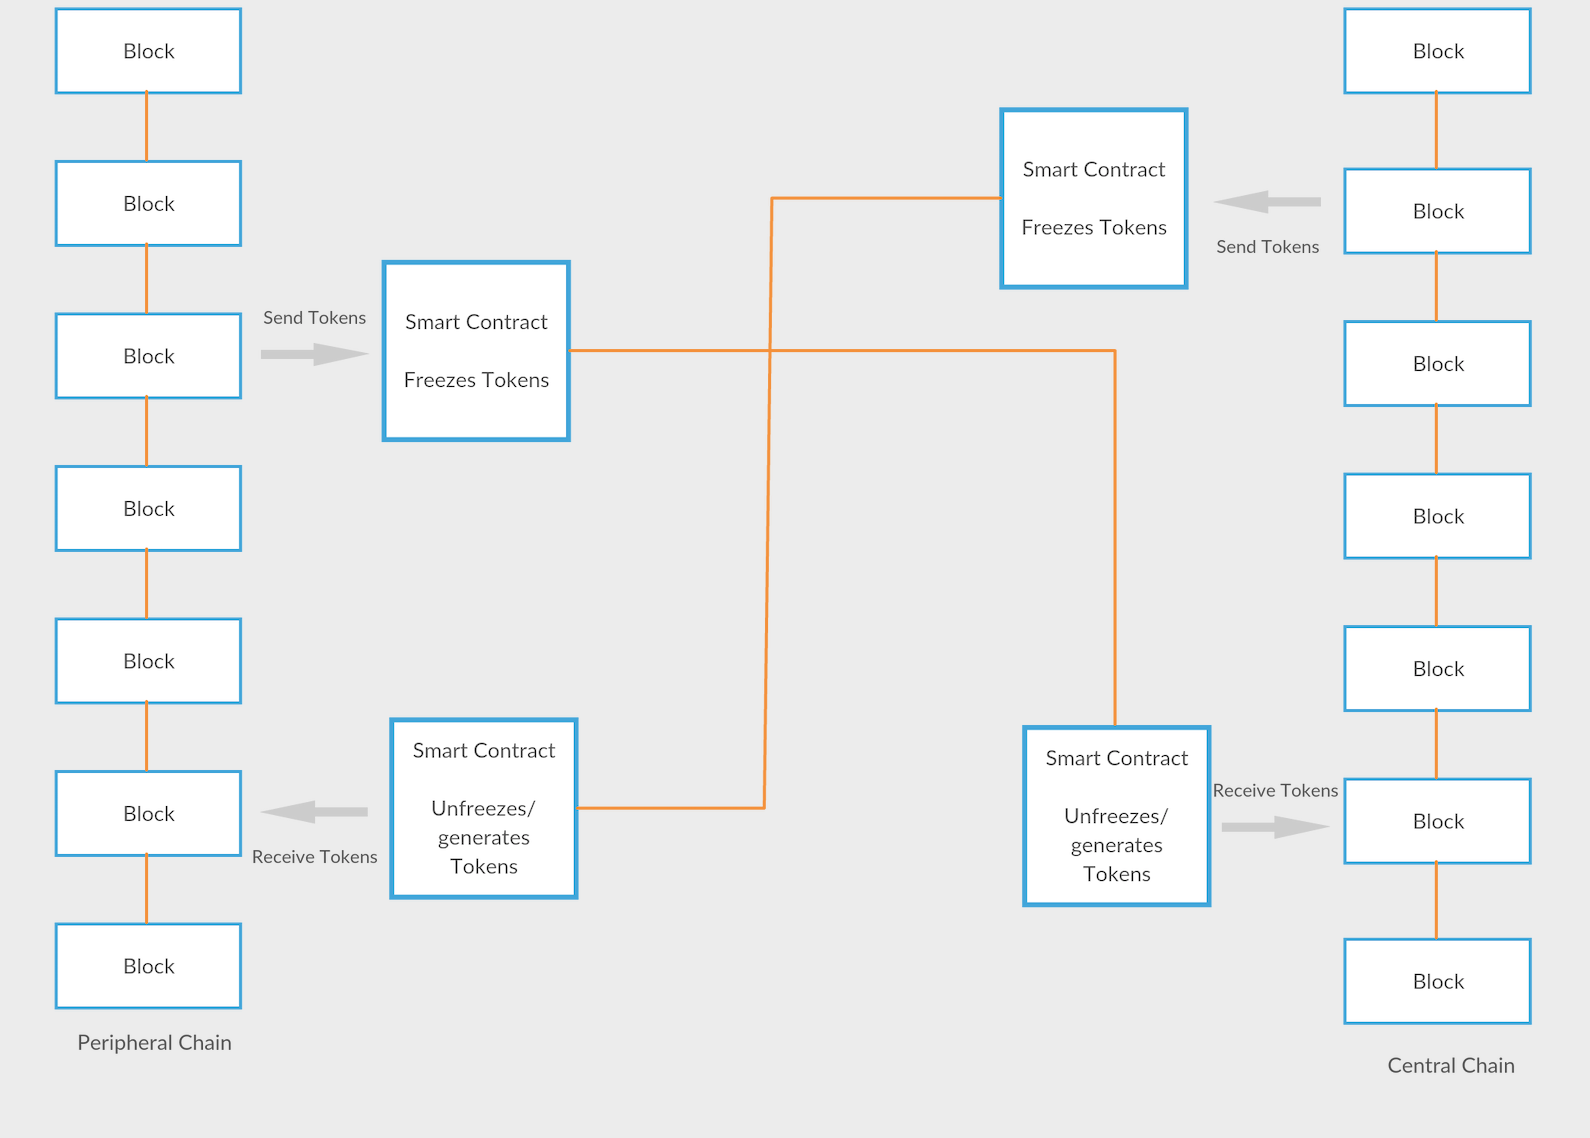
\includegraphics[width=\linewidth]{mirrored_blockchains.png}
  \caption{Mirrored Smart Contracts}
  \label{fig:smart}
\end{figure}

\subsection{Data Transfer and Transaction Validity}
The data fields mentioned in the previous section will need to be sent across from one token system to another. The ABCI facilitates this connection using sockets. This creates a standardised interface between the various token systems to exchange data. The NMZ chain also verifies whether the transactions are valid. Transaction validity is confirmed if the following conditions are met:
\begin{description}
\item[$\bullet$]the EC-Schnorr signature on the transaction is valid and a keyVerify() request from the cryptographic layer returns true.
\item[$\bullet$]the account has sufficient funds available for the transaction.
\end{description}

If the above conditions are met then the transaction is deemed valid and is eligible for further processing. The validation of other necessary information such as the destAddress and destAccount is completed in later stages. 
\section{Consensus Layer}
The consensus mechanism in the system described here is quite different from the consensus mechanisms that have been described in the literature review chapter of this thesis. The system utilises a permissioned blockchain. This makes achieving consensus relatively easier than popular mechanisms such as proof of work. The consensus mechanism here uses Tendermint which is a software for replicating state across machines\cite{TendermintTeam2018WhatDocumentation}.
\\
\\
Achieving consensus in permissioned blockchains is comparatively easier due to the fact that nodes are not anonymous and, therefore, the consensus mechanism to associate malicious behaviour with specific nodes. Since Tendermint is a blockchain independent consensus engine it requires certain arguments to be given as input\cite{}. The Tendermint Core interfaces with the system using ABCI to get the proper arguments and replicate the current state across all the active nodes.
\\
\\
The Tendermint core can be configured with the following parameters\cite{}:
\begin{description}
\item[$\bullet$ abci:]ABCI transport (socket|grpc). The system will use a socket configuration which is more widely used.
\item[$\bullet$ db\_backend:]Database backend for the blockchain and Tendermint Core state. The system will use leveldb because it is better at disk space utilisation \cite{}.
\item[$\bullet$ db\_dir:]Database directory. This will be set to the value ``\$TMHOME/data/chain\_ID", where chain\_ID is the value specified in the genesis.json file.
\item[$\bullet$ fast\_sync:]Whether to sync faster from the block pool. This field can be set to true or false depending on the need. If fast\_sync is enabled then the blocks are downloaded and the Merkle tree of the validators are checked instead of syncing the blockchain from genesis.
\item[$\bullet$ genesis\_file:]The location of the genesis file.
\item[$\bullet$ log\_level:] Defines the verbosity of the logs generated.
\item[$\bullet$ moniker:]Name of the node which is defining the configuration file.
\item[$\bullet$ priv\_validator\_file:]Validator private key file. The JSON file containing the validator's private keys.
\item[$\bullet$ prof\_laddr:]Profile listen address.
\item[$\bullet$ proxy\_app:]The ABCI app endpoint. The default value is Default: "tcp://127.0.0.1:46658"
\item[$\bullet$ consensus.max\_block\_size\_txs:]Maximum number of block txs. The maximum number of transactions in a block will be 5000 which will keep the block creation time to be approximately one block per second.
\item[$\bullet$ consensus.timeout\_*:]Various consensus timeout parameters
\item[$\bullet$ consensus.wal\_file:]Consensus state WAL. It recovers the system to a previous checkpoint in case of failure.
\item[$\bullet$ consensus.wal\_light:]Whether to use light-mode for Consensus state WAL.
\item[$\bullet$ mempool.*:]Various mempool parameters.
\item[$\bullet$ p2p.addr\_book\_file:]Peer address book.
\item[$\bullet$ p2p.laddr:]Node listen address.
\item[$\bullet$ p2p.pex:]Enable Peer-Exchange.
\item[$\bullet$ p2p.seeds:]Comma delimited host:port seed nodes.
\item[$\bullet$ p2p.skip\_upnp:]Skip UPnP detection.
\item[$\bullet$ rpc.grpc\_laddr:]gRPC Remote Procedure Call listen address (BroadcastTx only).
\item[$\bullet$ rpc.laddr:]RPC listen address.
\item[$\bullet$ rpc.unsafe:]Enable unsafe RPC methods.
\end{description}
\subsection{Genesis Block}
The genesis block is always hardcoded\cite{}. The genesis block acts a specification for other blocks to adhere to. In Tendermint, the parameters in the genesis block have to be specified, in the Genesis.json file. This file contains the following fields:
\begin{description}
\item[$\bullet$genesis\_time:]Official time of blockchain start. The value for this field will be generated automatically by the system based on the Unix timestamp.
\item[$\bullet$chain\_id:] ID of the blockchain. This must be unique for every blockchain and will be the ID generated by the cryptographic layer during the chain initialisation.
\item[$\bullet$validators:] This is a list of validators whose accounts will exist from genesis. Each validator in the list of validators contains the following fields:
\begin{description}
\item[$\bullet$pub\_key:]The first element specifies the pub\_key type. The second element is the pubkey bytes.
\item[$\bullet$amount:]The validator’s voting power.
\item[$\bullet$name:]Name of the validator (optional).
\end{description}

\item[$\bullet$app\_hash:]The expected application hash (as returned by the Commit ABCI message) upon genesis. If the app hashes do not match, a warning message is printed. This field is present at the end of the validator list.
\\
\\
\end{description}
Appendix C contains a sample genesis.json file for reference. The configuration of the Tendermint core to achieve consensus concurrently on the NMZ main chain and the logging chain is the most challenging part of the configuration the consensus engine.
\section{Cryptographic Layer}
The cryptographic layer is essential for enabling the interoperability of the multiple token systems. The important function is the generation and maintenance of the public and private keys across the system. The cryptographic layer is responsible for generating all the public and private key pairs for each peripheral blockchain associated with the central blockchain.
\\
\\
The cryptographic layer uses the EC-Schnorr digital signature algorithm instantiated with the sepc256k1 elliptic curve to generate key pairs. Every time a proposal for the integration of a new token system is generated by an admin user, the cryptographic layer is invoked to generate the public key address of the peripheral chain and add it to the smart contract proposal. The private key is kept confidential until the new token system has been fully incorporated. If the proposal for incorporation is accepted, the cryptographic layer adds the private key to the smart contract on the peripheral blockchain before deploying it. Once the smart contract is deployed onto the peripheral chain, the private key is deleted from the system. However, if the proposal is by the voting process, then the cryptographic layer deletes all records of the private or public key of the proposed token system. It pushes the details across to the logging system to keep a secure record of the activity.
\\
\\
The central Numiz(NMZ) blockchain relies on the cryptographic layer to access the public addresses of the token systems during the process of the token transfer across different chains. Figure \ref{fig:6} shows the interaction between the central blockchain and the cryptographic layer in the following use cases:
\begin{description}
    \item[$\bullet$ Request to generate keys (keyGen()):] Before a new token incorporation proposal, the blockchain to be deployed needs to have a public key attached to the smart contract. The central chain requests the generation of new keys from which the public key is attached to the smart contract and the private key is sent to the temporary key database until the proposal is voted on.
    \item[$\bullet$ Key Verification Request (keyVerify()):] The processing of transactions requires the central chain to verify the blockchains that are parties to the transaction. This involves retrieving the public keys to verify the certificate that is attached to the transaction data packet. This verification is a security requirement such that the system does not accept transactions from unverified sources. 
\end{description}
\begin{figure}
  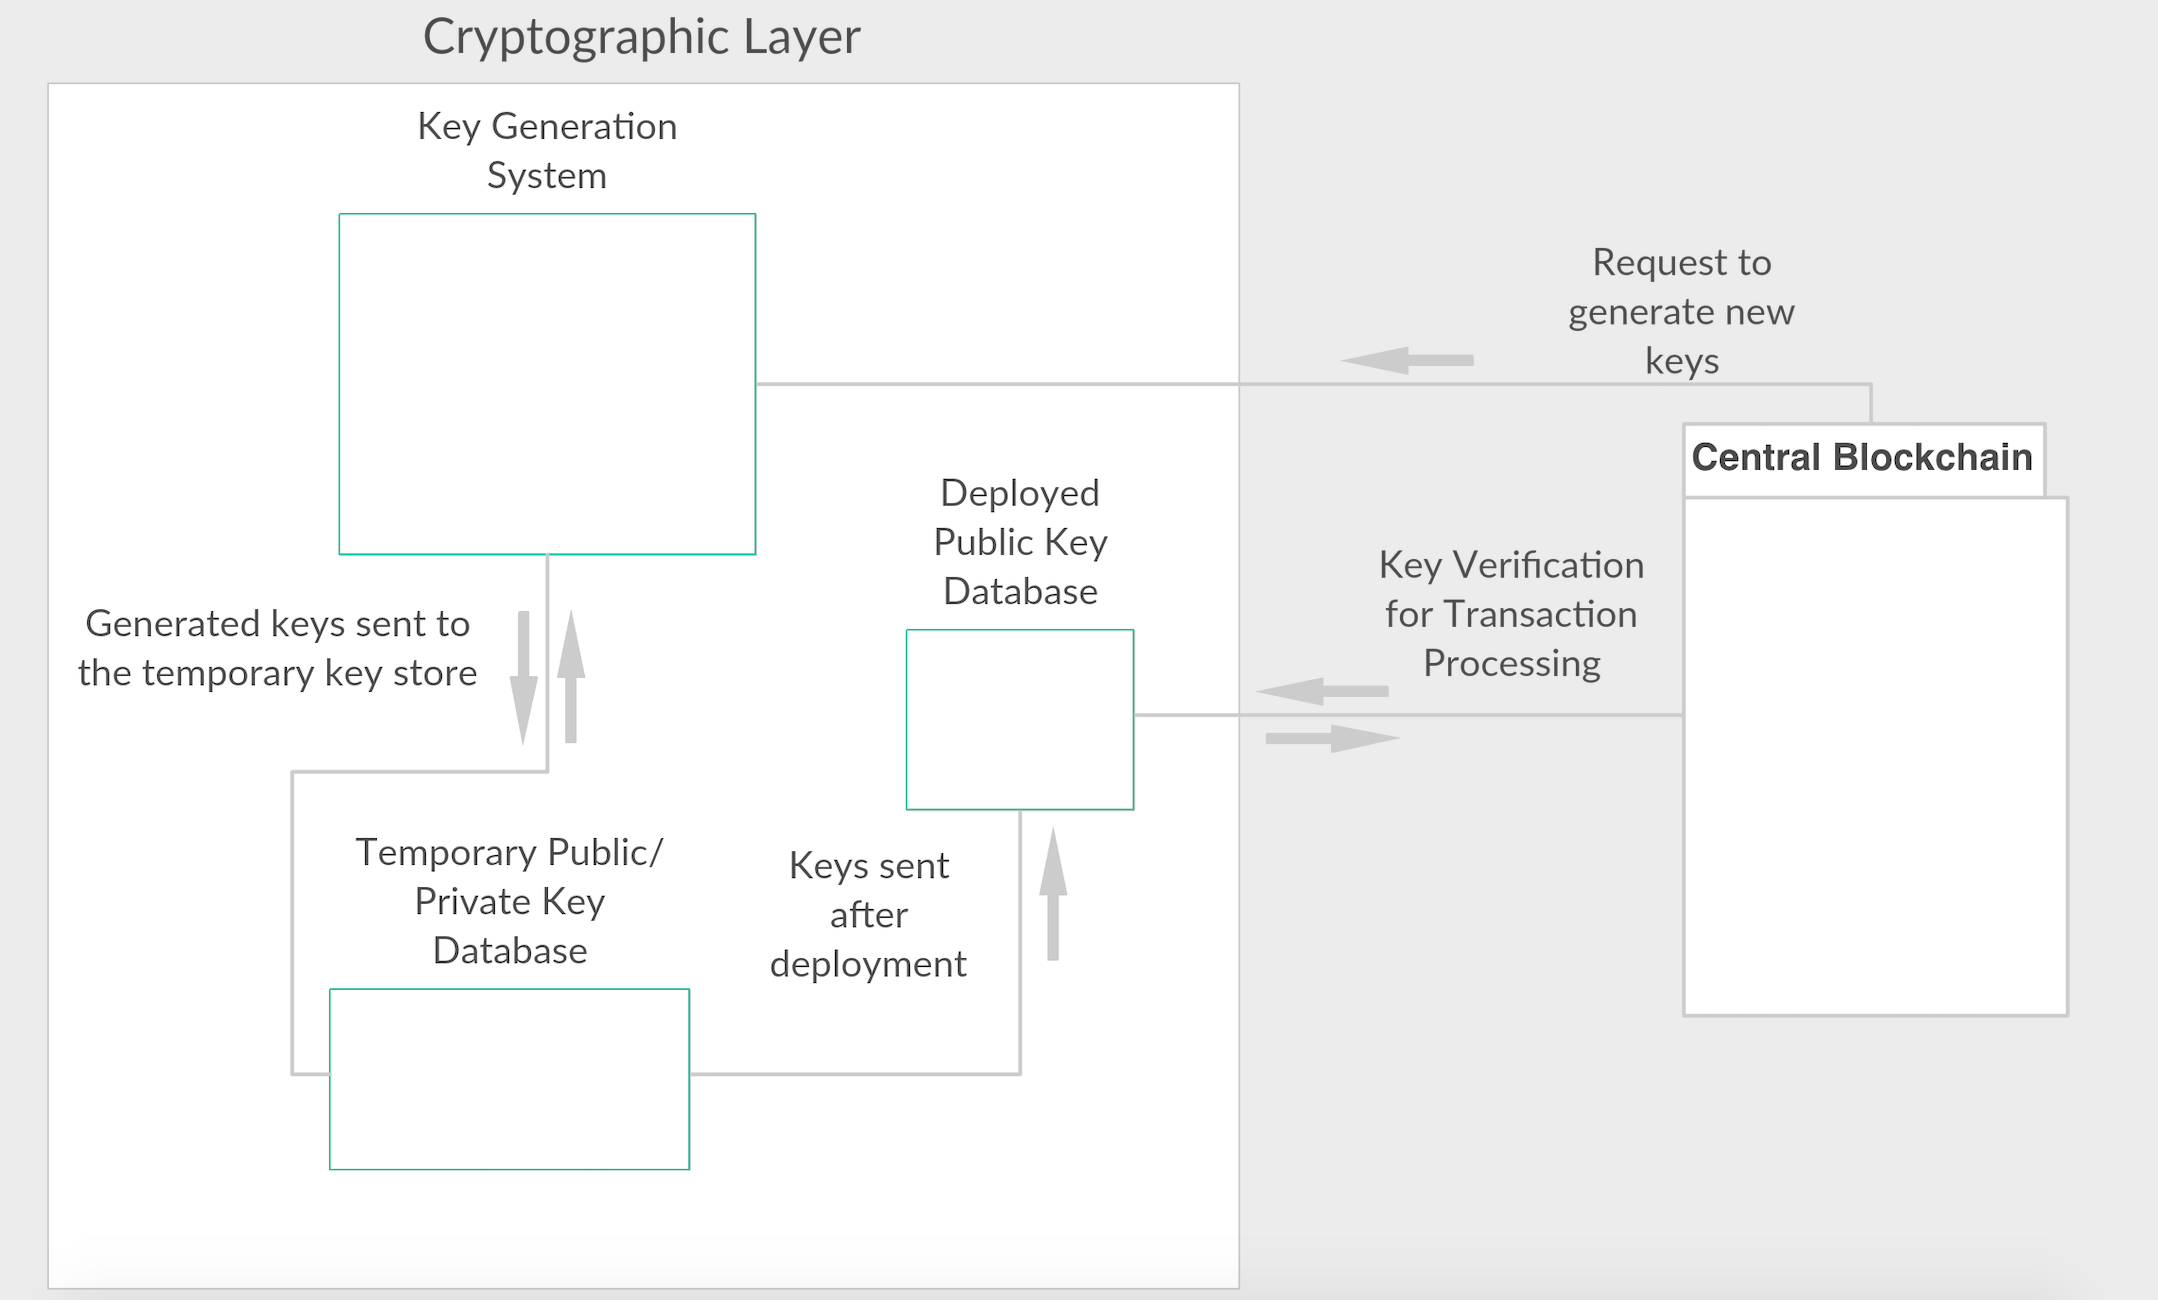
\includegraphics[width=\linewidth]{cryptographic_layer.png}
  \caption{Crytographic Layer Interaction with Central Blockchain}
  \label{fig:6}
\end{figure}
\section{Logging Layer}
The logging system is a unique component in the architecture of the proposes system. It is completely independent of the central blockchain even though they work concurrently with a time gap of no more than 6 seconds. It maintains a separate blockchain specifically for logging activities. This is perhaps the most unique feature which is much needed in a system of this nature. Figure \ref{fig:6} shows the design and architecture of the logging layer. It has a completely decentralised blockchain with an independent Tendermint Consensus engine.
\\
\\
The logging system blockchain is concurrent and self-governing. Self-governing implies that it is a decentralized blockchain with every node having equal voting rights. Unlike, the central blockchain where its servers and the overloading system have more authority over the other nodes in order to keep the system functional and scalable. The central blockchain also has mining pools which further compromises on the centralisation of the architecture. The logging blockchain does not need to have multiple mining pools for the purpose of parallel processing because it only logs the headers of the Merkle tree, taken from the central blockchain. The headers are scanned through the security system to ensure that there are no inconsistencies present.\\
\\
The security layer ensures that the headers logged are consistent with the central chain. It could be stated that the security layer acts as a consensus layer between the logs and the central blockchain. The security layer resembles a consensus mechanism between the two independent blockchain systems.
\begin{figure}
  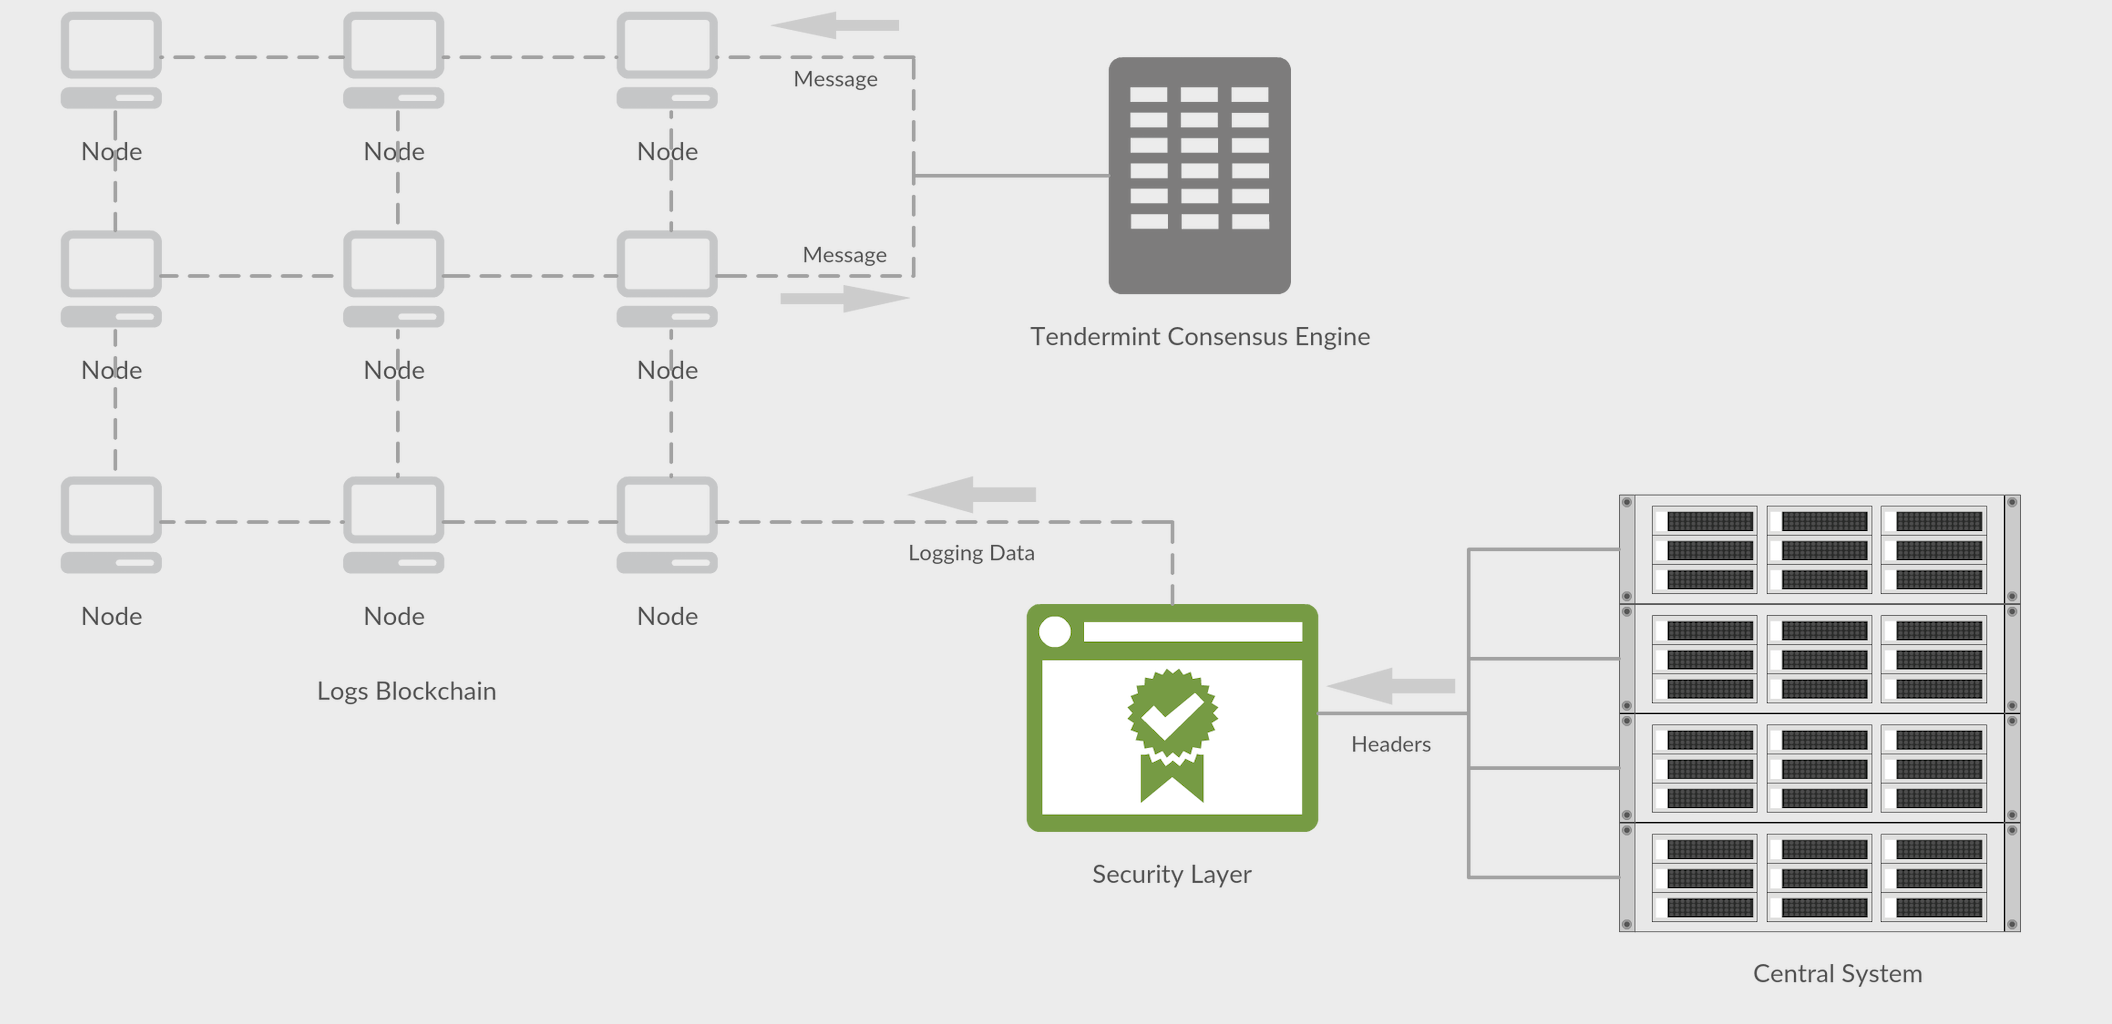
\includegraphics[width=\linewidth]{logging_layer.png}
  \caption{Logging System Architecture}
  \label{fig:2}
\end{figure}

\section{Security Layer}
 The security layer ensures that potential security breaches are detected by the system. It uses machine learning classifiers to detect whether each operation attempted on the system was malicious. All data logs are scanned through the security layer before being permanently pushed to the logs blockchain.   
\\
\\
The machine learning model used in malicious activity detection is based on the research published by Prateek Dewan et all. on Detecting Malicious Content on Facebook\cite{Dewan2015DetectingFacebook}. The model will be modified in order to detect malicious activity on blockchain transactions instead. Another feature of the security layer is the ability to cross check the Merkle tree headers in the logs blockchain to detect any discrepancies. The security layer acts as a consensus mechanism and interface between the logs layer and other components of the system.
\section{Backup Layer}
Blockchain systems are usually highly redundant, when it comes to data storage as all the nodes are redundantly storing all the data\cite{}. However, in production-grade blockchain systems such as the one being described here a backup system is essential, particularly when deployed in banking, finance, and supply chain industries. The backup layer will be activated when the number of active nodes falls below the MOL. The MOL in this case is 10000 active nodes, however, this parameter could be redefined in the configuration file. Activation of the backup layer puts the system in a backup mode where the components rely on the backup data storage servers for data retrieval and consensus. This backup data and bandwidth are used for elements of transaction processing that require data retrieval from the backend. 
\\
\\
The backup layer is activated as soon as the total number of nodes goes below the initial 10000 available active nodes. Active nodes are defined as the nodes in the network that are involved in the transaction processing and consensus mechanism. The system pings nodes every 600 milliseconds and creates a bitmap of the active nodes. A particular bit in the bitmap is of value 1 or 0 depending on if the particular node is active during the ping. The system has a particular arrangement of nodes in incereasing order of the timestamp of when the particular node was first registered. This information combined with the bitmap generated during each pinging cycle makes it easy to determine a variety of network information such as the number of active nodes, public addresses of these nodes, and their involvement in transaction processing.

\subsection{Storage}
The backup layer is comprised of a data server and a storage layer. The storage layer contains one main database and three mirror storage units. The storage on the database is a snapshot of the global state of the blockchain system taken once every 100 blocks. This snapshot is then copied across the three mirror storage units. The design of the storage layer is given in figure \ref{fig:3}. The backup mirrors are used in case of the failure of the main storage layer, which itself is only activated in case of the total number of the active nodes falling below the minimum operable linnit (MOL). Therefore, the likelihood of the backup mirrors ever being used is extremely low. The backup system exists to increase the integrity and robustness of the system.

\subsection{Server Nodes}
The server nodes get activated as soon as the number of active nodes in the system falls under the MOL which is 10000 nodes. The server nodes scale according to the number of nodes required to get the system back to the MOL. For example, if the total number of active nodes falls to 9986 nodes then the number of server nodes in the backup layer will be scaled to 10000 - 9986 = 14 nodes.
\begin{figure}
  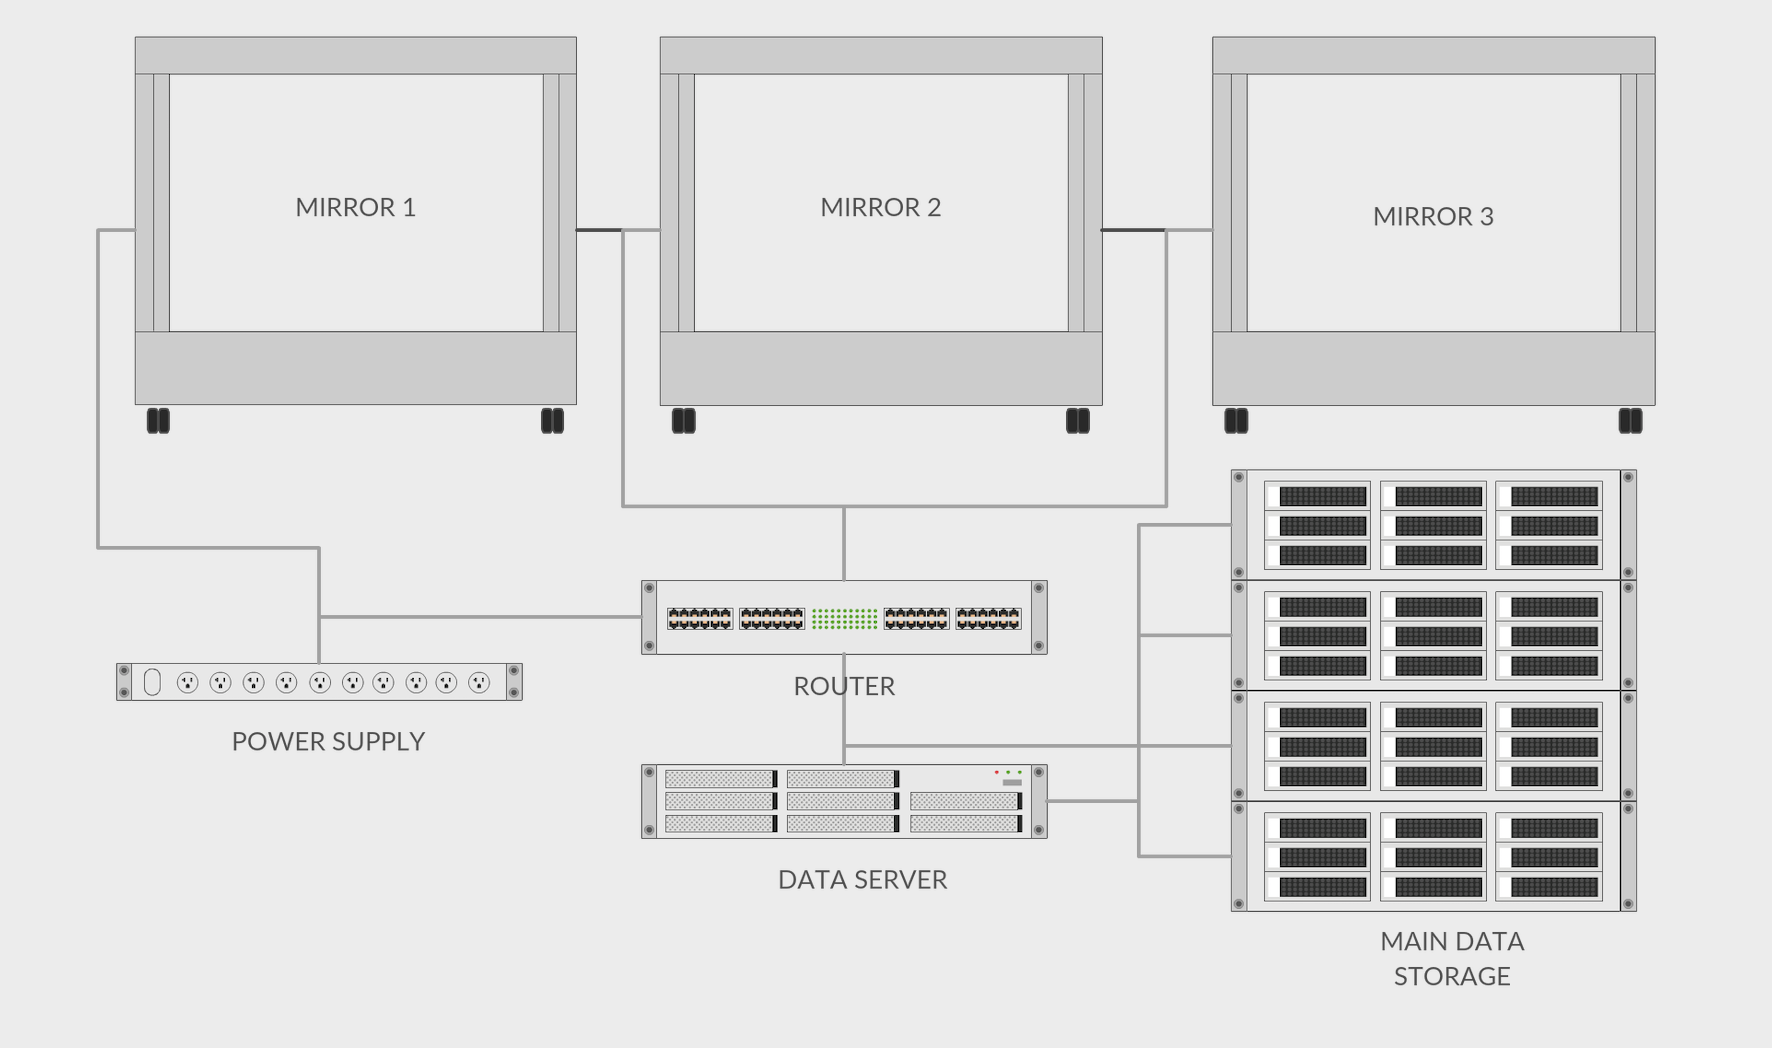
\includegraphics[width=\linewidth]{storage_layer.png}
  \caption{Storage Layer Architecture}
  \label{fig:3}
\end{figure}

\section{Network Layer}
The network layer is crucial as it allows the system to achieve high scalability without compromising on security. The network layer is the backbone of the scalability and parallel processing ability of the system. The network layer has the following functionality:
\begin{description}
\item[$\bullet$] segregate the entire mining pool into multiple smaller shards for parallel processing of transactions
\item[$\bullet$] allocate new nodes into mining shards
\item[$\bullet$] allocate transactions to one of the valid shards
\item[$\bullet$] confirm the validity of the transactions 
\item[$\bullet$] queue transactions when all the shards are busy
\item[$\bullet$] retrieve transactions from the processing queue and allocate them to an appropriate mining shard for processing
\end{description}
\subsection{Sharding of the Mining Pool}
The mining pool in the system is divided into multiple shards enabling the shards rto process transactions in parallel. There are some important concerns that need to be addressed before the algorithm for dividing the mining pool into shards can be implemented. One of the main concerns is to find an effective ratio between the number nodes in a sharded pool and the total number of nodes. The ratio of the number of nodes in each pool, n, to the total number of nodes, N, is called the pool ratio, $\phi$. $\phi$ varies directly with the total number of nodes in the pool. The number of nodes in each pool becomes higher if the total mining pool size increases and vice-versa. However, the increase or decrease is not a direct one-to-one correlation. Initially, each pool will begin with 1000 nodes while the total number of nodes will be set to 10 times that. Any increase in the total number of nodes will trigger the addition of the nodes sequentially into each shard. The new nodes are continually added to the shards until each shard reaches the rearrangement point. The rearrangement point is defined as the increase in the number of nodes to 1/5th of the total number of nodes. At the rearrangement point, the system automatically dissolves all the shards and starts the process of rearranging the nodes by increasing the number of shards. This is done in order to keep the pool ratio within a certain range. The process of rearrangement also ensures that there is an effective increase in the number of mining shards with the increase in the number of nodes. This has scalability and efficiency advantages.
\\
\\
The pool ratio is defined as follows:

\[\phi = n/N\]

The value of $\phi$ is the average value taken from each individual pool. The initial value of phi is approximately 1000/10000 = 0.1. This value varies as nodes get added. Every rearrangement of the mining pools resets the value of $\phi$ as close as mathematically possible to the default value of 0.1.


\section{Smart Contract and Virtual Machine Layer} 
The system has a smart contract processing layer that contains a virtual machine for processing various transactions and computations. The virtual machine is capable of processing any kind of computational operation in the form of transactions. The virtual machine will be a heavily modified version of the Ethereum Virtual Machine (EVM). The virtual machine executes bytecode code in binary form. The smart contract layer has an integrated compiler that converts code written in various popular languages such as JavaScript or Python to bytecode code which is a form of binary code that natively runs on the Virtual Machine.
\\
\\
The smart contract and the virtual machine have two separate parts, as stated below:
\subsection{Smart Contracts}
The smart contracts can be written in any language. The compiler converts the languages into virtual machine code or bytecode which can run natively on the system. This makes the virtual machine compatible with various systems.
\subsection{Virtual Machine}
The core of the virtual machine is a standard EVM core which is a simple stack-based architecture \cite{Wood2018ETHEREUM:LEDGER}. 
\section{System Integration}
 Proper integration is crucial for the functioning of the system of this complexity. Figure \ref{fig:3} shows how the different components of the system operate in conjunction with one another. The peripheral blockchains are all connected to the system through a data traffic router. All the data traffic passes through the smart contract layer which contains the mirrored smart contracts for each peripheral blockchain. The smart contracts layer is the entry point to the NMZ chain for the multiple peripheral blockchains.
\\
\\
The central blockchain is isolated from the peripheral system. The central chain system is comprised of the central chain, network layer, security and logging layers, consensus engine, cryptographic layer, and the backup system, all connected to each other using a data traffic router. The overview of the entire system and its integration is described here. The central chain system is only applicable to inter-chain transfers.
\subsection{Data Flow}
The data flow begins with one of the peripheral blockchain systems initiating a transaction. The request goes through the router to the NMZ chain's corresponding smart contract. The smart contract verifies the validity of the transaction by using a connection to the cryptographic layer. The transaction data is then sent back to the network layer for allocation to a mining pool or the transaction queue if no pools are currently available. The transaction is then sent back to the NMZ chain for processing. After the processing of every 5000 transactions, the data is bunched together in a block. A copy of the block data is sent to the Tendermint consensus engine and the logging layer. The logging layer has a separate Tendermint consensus engine. Finally, the security layer verifies whether the logging blockchain and the NMZ chain have exactly the same copy of the data. This is done by comparing the hashes of the corresponding block headers from the two blockchains. This achieves consensus among the independent components of the architecture.
\begin{figure}
  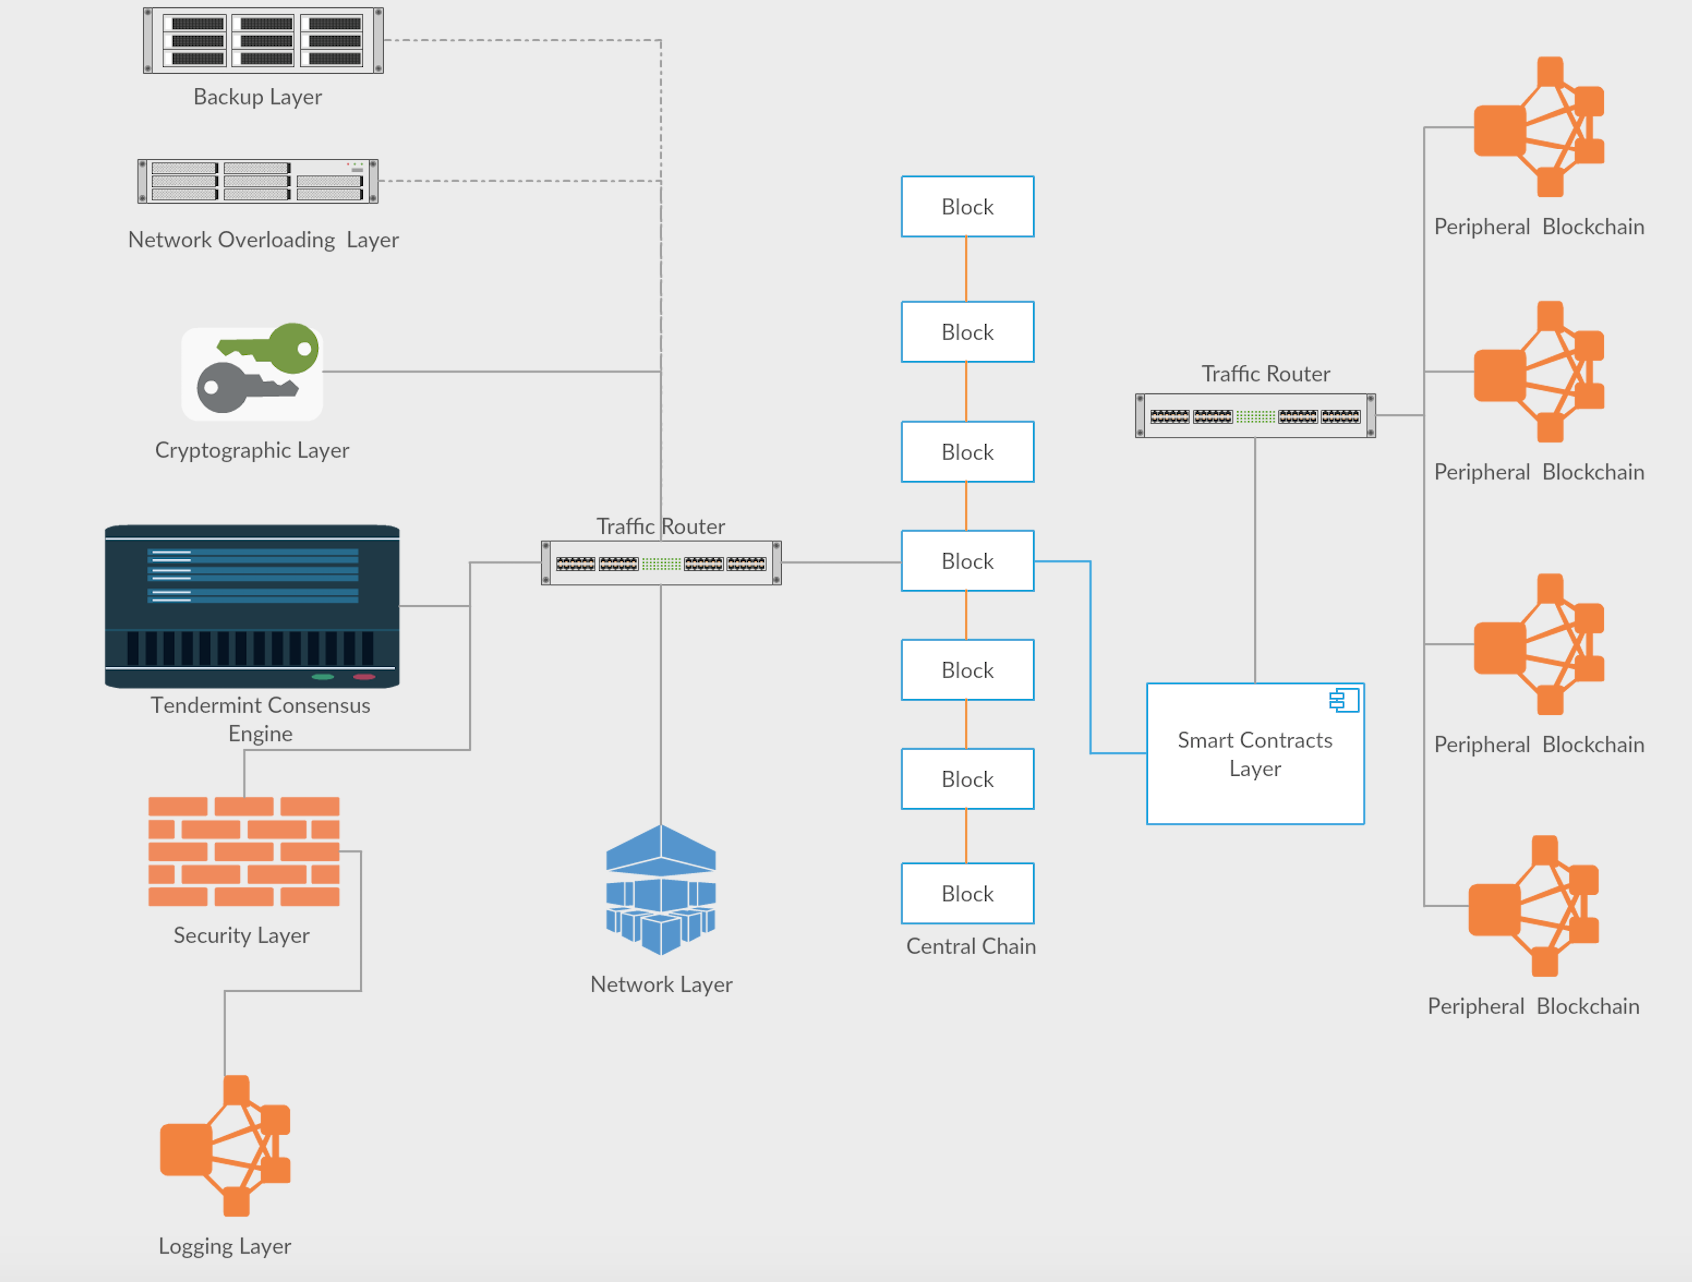
\includegraphics[width=\linewidth]{system_overview.png}
  \caption{System Architecture}
  \label{fig:3}
\end{figure}
\chapter{Discussion}
\label{chap:Discussion}
The previous chapters have presented the system architecture and implementation of a blockchain solution which is scalable and interoperable with multiple blockchain systems. This chapter discusses some of the potential issues that might be present in the system design and implementation. It also discusses the potential industry use cases for the system and possible issues that might arise during integration.

\section{Incomplete Design and Implementation}
The design and implementation of the system are not comprehensive. Some of the specific details of the implementation such as the detailed specifications for the data transfer between the corresponding mirrored smart contracts, and the code used in such contracts is missing. This aspect of the implementation of the system requires further research. The project on a system design level is comprehensive, however, each component of the system is a system within itself. A complete design and implementation for each specific component of the system would have been outside the scope of this project. The specific details would have taken much longer to research and implement and would have made this thesis much longer than the scope or time-frame permitted.
\\
\\
Even though the current form of the system is not specific and detailed enough for immediate adoption, it is a good initial architecture for such a system to be built on. The minor inconsistencies in design and specification can be perfected over time with use. Furthermore, this thesis showcases the fact that such a blockchain architecture is possible to implement, if more research and development is done in this area. This thesis aims to provide a decent starting point for such research and development.
\section{Generation of New Tokens}
The system has a smart contract layer that has corresponding mirrored contracts on the central blockchain which facilitate the transfer of tokens across multiple peripheral blockchains. The way that those smart contracts work is by freezing the tokens in the sending blockchain's smart contract account and releasing the equivalent amount of tokens in the receiving blockchain. The only issue with such an approach is the limitation due to the availability of sufficient funds in the receiving chain's smart contract account. For example, an account holder on a sending Bitcoin peripheral blockchain, sends a transaction of 100 Bitcoins to an account holder on the receiving peripheral Ethereum blockchain. The system calculates the conversion of 100 Bitcoins to Ethereum, which for example is 6000 Ethereum tokens. The smart contract on the Bitcoin blockchain initiates the transaction and sends the tokens across to the corresponding Ethereum contract via the central NMZ chain. However, the corresponding Ethereum contract account does not have enough Ethereum to be able to transfer the tokens to the receiving account. This results in a reversal of the transaction, even though the sender had sufficient funds and the transaction was otherwise valid. 
\\
\\
The problem mentioned above creates a major issue with the overall reliability of the system. The failure of transactions beyond any fault on the users' part will result in being a significant source of frustration, potentially affecting the adoption of the system. The potential solution to this issue and future developments are discussed in Chapter \ref{chap:FutureWork}.
\section{Potential Use Cases}
The system has been designed with a modular and cross-compatible architecture, allowing for a multitude of industry use cases such as in banking, finance, supply chain management, accounting, and other organisations that have multiple parties involved in a business transaction. 
\\
\\
One example use case is the remittance system within the banking infrastructure. Currently, the banking systems use numerous middleware and complex routes in case of  cross-continent fund transfers. In most cases, due to the complexity of such a transaction, it usually takes days for the remittance to be successfully processed. Banks use processing services such as MasterCard and VISA for card payments and Society for Worldwide Interbank Financial Telecommunication (SWIFT) messages for international funds transfers\cite{2018SWIFTTransferWise}. The NMZ system can simplify the processing of such transactions. The banks around the world could have their own internal blockchains which will be connected to NMZ. The exchange of funds among those bank blockchains could be facilitated via the NMZ chain. 
\section{Compatibilty with Existing Infrastructure}
The system has been designed to be compatible with most existing industry architectures although it might have integration issues with existing legacy software\cite{JohnLamb2008LegacyEnterprise}. Legacy software is still used in most banking infrastructures\cite{JohnLamb2008LegacyEnterprise}. To complicate matters most of this software is closed source and proprietary, making it harder to get the system specifications of such software. Moreover, unless there is a partnership agreement with the client organisation, it is impossible to know the specifications of their software. This makes the process of making the system completely compatible with all such software architectures, impossible. However, the system has been designed with modularity and cross-compatibility in mind. The system can be easily modified to suit the certain configurations and needs of each client infrastructure, once the specifications of their infrastructure are made available.
\section{Adoption Risk}
The system has been designed to be used in large-scale organisations and infrastructures such as the banking system or the supply chain management. These infrastructures are usually controlled by a few major corporations such as the Commonwealth Bank and ANZ in the case of banking, or Maersk and DHL in the case of supply chain and logistics. These organisations are usually very risk-averse\cite{Gorter2011DNBInvestors}. The completely new architecture will change the way they conduct business and, therefore, may be extremely hard for them to adopt and integrate into their workflow.
\\
\\
The system has not yet been tested in real-world applications. The lack of sufficient testing may deter these large organisations from taking the risk of integrating such a system into their architecture. This is a paradoxical situation because improvements to system reliability and compatibility relies on increased adoption and optimisartion over time. Unless these client organisations release their transactional data or system specifications, it is not feasible for the system to be optimised for its different use cases in different industries.

\chapter{Conclusions}
The widespread adoption of blockchain systems in commercial applications has been hindered by the limited scalability of such systems\cite{GavinWood2018POLKADOT:FRAMEWORK}. Interoperability is another problem, whereby, different blockchains cannot communicate with each other for transactional purposes\cite{GavinWood2018POLKADOT:FRAMEWORK}. Both of these factors have practically limited the transaction throughput to approximately 30 transactions per second\cite{GavinWood2018POLKADOT:FRAMEWORK}. The goal of the project was to create a framework for multiple blockchain ecosystems to be able to transact among each other. To approach this problem, different attempts to scale blockchains were evaluated. An architecture for a system which will facilitate the interconnectivity of blockchains was designed using good software engineering practices. This chapter provides a conclusion to all that this project has been able to accomplish.  
\\
\\
A literature review revealed the multiple approaches to solving the problem being addressed in this paper. Some of those attempts are the foundation for the system that has been presented in this thesis. The core system is based on the architecture of Ethereum. The approach to scale transactions by dividing the entire mining pool into smaller pools is based on the approach taken by Zilliqa. The approach to connecting multiple blockchain systems with a central blockchain is based on Cosmos. The consensus engine is a configuration of Tendermint. The other components of the framework such as the logging system and the backup architecture are original contributions.
\\
\\
It was discovered during the literature review that most blockchain systems have not been designed with consideration given to good software engineering and testing practices. The explanation given in most systems was found to be inadequate. Proper system design documents such as Software Requirements Specifications (SRS) and System Test specifications of such systems were not found. Therefore, one of the important achievements of this thesis was to create proper requirements and test documentation for the system. The process began by starting with the SRS document. The requirements found in the SRS were used to create a test specification.  A Test Driven Development (TDD) approach was taken in the development of the architecture.
\\
\\
The requirements gathered and the test specifications developed in the first half of the project were used in the system design and implementation process. The main accomplishment of the project is the framework presented in Chapter \ref{chap:System Implementation}. The framework facilitates the inter-connectivity of multiple blockchains. The system implementation also includes an approach to improve the scalability of the blockchains by increasing the transaction throughput. This was achieved by dividing the entire mining pool into many smaller pools enabling transactions to be processed in parallel. The system integration design presented at the end of Chapter \ref{chap:System Implementation} shows the complete design overview of the system. 
\\
\\
The system has several shortcomings. One of those is the inability of the system to create new tokens if the smart contract account lacks sufficient funds for a transaction. This issue has been addressed in Chapter \ref{chap:Discussion} and \ref{chap:FutureWork}. An alternative approach to creation of new tokens by using tokens other than the native token is a feasible approach. The system has potential applicability in production grade, high-risk software infrastructures such as the banking network and the supply chain management. 
\chapter{Future Work}
As described in Chapter \ref{chap:Discussion}, it has been mentioned that the systyem has not been implemented. There is a lack of specific information regarding the deployment of the smart contracts. Furthermore, there is also an issue of token generation when there is a lack of funds for a remittance. This chapter discusses future work which would benfit form focussing on the follwoing areas.

\section{Generation of New Tokens }
The inability of the system to generate new tokens is a critical issue. There are a few potential ways this issue can be approached. One of the potential solutions is the use of coloured coins. Ecosystems such as Ethereum and Bitcoin have the ability to support alternative tokens generated by smart contracts\cite{DigitalDraglet.com}. Instead of using the native tokens of the blockchain system which cannot be generated by these smart contracts, the mirrored smart contract accounts can use alternative tokens. These tokens can then be converted to the native token of the blockchain using a token exchange. 

\section{Smart Contract Specification}
The specifications for smart contracts proposed in this system have not been implemented and the code has not been finalised. Code that is going to be implemented in the smart contract has to be specified. The future work on these specifications will improve the utility of the system.
\\
\\
The details and specifications regarding the communication protocol between the mirrored smart contracts need to be more explicit. Issues may arise during the implementation that will need to be addressed in the smart contract specification.
\section{Closing Remarks}
The system implementation is incomplete and has several issues that need to be addressed. However, this thesis forms a good foundation for implementation of such a system. If more work is directed into parts of the system that lack details, the system could be a commercially successful blockchain. 
\label{chap:FutureWork}
\chapter{Abbreviations}
\label{chap:abbreviations}

\begin{tabbing}
\hspace*{4cm}\= \kill
ABCI \> Application Blockchain Interface\\
ASIC \> Application Specific Integrated Circuits\\
AWS \> Amazon Web Services\\
BFT \> Byzantine Fault Tolerance / Tolerant\\
DDoS \> Distributed Denial of Service\\
DS \> Directory Service\\
ECDSA \> Elliptic Curve Digital Signature Algorithm\\
EVM \> Ethereum Virtual Machine\\
GDPR \> General Data Protection Regulation\\
IBC \> Inter-blockchain Communication\\
ILP \> Interledger Protocol\\
MOL \> Minimum Operable Limit\\
NMZ \> Numiz\\
PBFT \> Practical Byzantine Fault Tolerance / Tolerant\\
PKI \> Public Key Infrastructure\\
PoW \> Proof of Work\\
RLP \> Recursive Lenght Prefix\\
RPC \> Remote Procedure Call\\
SHA \> Secure hashing Algorithm\\
SRS \> Software Requirements Specification\\
SWIFT \> Society for Worldwide Interbank Financial Telecommunication\\
TDD \> Test Driven Development\\
TSP \> Tendermint Socket Protocol\\
UTXO \> Unspent Transaction Output\\
\end{tabbing}

%\phantomsection \addcontentsline{toc}{chapter}{Index}
% \renewcommand{\baselinestretch}{1} \small \normalsize
% \printindex

\appendix
\chapter{Project Plan}
\section{Abstract}
Blockchain scalability is one of the major problems that need to be addressed in the entire blockchain space. Of the many approaches for scaling blockchains, facilitating intercommunication of smart contracts among multiple blockchains while maintaining consensus is a promising approach. This paper lays the project road map for the research regarding a novel protocol for intercommunication among multiple private Ethereum blockchains. The paper also discusses how this protocol can be demonstrated using an app built on react-native that could interface with the blockchains and help facilitate and demonstrate this interconnectivity protocol. Moreover, the paper provides a detailed project plan along with background and literature review, approach and methodology, intended research outcome, and expected impact of the outcome.
\section{Introduction and Background}
Blockchains have an immense potential to revolutionize the way the internet is being used today. Blockchain and Distributed ledger technology will lead the way into what is being termed as Web 3.0 [1], in which there is no point of central control like Google, etc., and in which data is owned by the peers and not the big data firms. Until now, blockchains and distributed ledger technology have only been synonymous with Bitcoins and other cryptocurrencies. However, this new technology has numerous potential applications in many different fields such as supply chain management, distributed computing, and many other applications that still need to be discovered.
\\
\\
Blockchains available at the moment are far away from being massively scalable in order to cater for these potential applications on a global scale. With an average of about 15 transactions per second [2], popular blockchains like Ethereum are far from being scalable. Numerous attempts have been made in order to scale blockchains and improve the transaction rates. Just in comparison with other payment platforms such as VISA and Mastercard, VISA does on average 1667 transactions per second with a peak capacity of about 56000 transactions per second [3]. Similarly, Mastercard processes about 2834 transactions per second on average and has a peak operating capacity of about 95000 transactions per second [4]. However, it is important to note that VISA and Mastercard are platforms meant only for payments processing. A public blockchain such as Ethereum can run DApps. DApps are distributed applications that can run on the EVM, the Ethereum Virtual Machine, which is a giant virtual computer that gathers its computing resources from all the computers running on the Ethereum Public Network. Each DApp is essentially a suite of smart contracts that work together to achieve the functionality of the DApp in a completely decentralized and peer-to-peer network [5]. Smart Contracts are autonomous agents on the blockchain that execute a transaction when certain conditions are met [6]. Each request on a DApp is executed as a smart contract transaction on the blockchain. As of writing this, the Ethereum public blockchain has 1657 decentralized apps and the number is rapidly increasing every day. With a transaction rate of about 15 transactions per second, this creates a serious bottleneck on the blockchain for running transactions.
\\
\\
A blockchain or a distributed ledger is a secure mechanism to run these transactions and sync the data across all the nodes in the network in order to make it secure and tamper proof. This same mechanism that makes blockchains, primarily so secure also make them massive unscalable and slow. There are many ways in which this problem of transaction scalability of blockchains can be solved. One of the solutions is to enable facilitation of smart contracts to be able to communicate among themselves while running on separate blockchains. Thus, each DApp could run on its own separate blockchain while communicating with smart contracts on multiple blockchains to achieve consensus of data, consensus being the main factor that makes blockchains tamper resistant. This project is going to explore possible solutions to this smart contract communication problem among separate blockchains, in a fast and secure way, so as to maintain the fault tolerance capability that these blockchains exhibit.
\section{Project Scope and Deliverables}
The project title is quite broad and can be applied to a lot of different blockchains and other distributed ledger technologies that have smart contract functionality. Some of these possible blockchains are Ethereum, Hyperledger Fabric, Hyperledger Sawtooth, Cosmos, etc. However, in order to keep the scope of this project specific and achievable, the project is going to be focused on developing such a seamless smart contract communication protocol on multiple Ethereum private networks. Developing, a generic protocol such as TCP/IP for smart contract communication would be the ideal outcome but might turn out to be a daunting task for a project that has a time scope of about 15 weeks.
\\
\\
Therefore, in order to keep the scope of the project specific and achievable, the project would aim to create a protocol for communicating messages across smart contracts on multiple Ethereum private networks. However, creating a generic protocol is still on the table, and if the timeline of the project permits then, a large amount of work will be put into delivering a generic protocol for platform-independent communication among smart contracts on multiple blockchains, such as Ethereum, Hyperledger Fabric, Hyperledger Sawtooth, or any other blockchain platform that has a Virtual machine and smart contract capability.
\\
\\
The questions that would need to be addressed in this thesis as deliverables would be the following:
\begin{description}
\item[$\bullet$]What is a secure way to encrypt a message so that it could be sent out of the blockchain without being subject to a man-in-the-middle attack?
\item[$\bullet$]How can the multiple blockchains achieve consensus of data?
\item[$\bullet$]How can a relay blockchain be secure without being the single point of failure?
\item[$\bullet$]How much information is needed to be communicated among the smart contract suites of different blockchains?
\item[$\bullet$]What is best approach to make sure that the security of the information is not compromised during communication?
\item[$\bullet$]What will be the improvement in the transaction throughput, once the technology is implemented?
\item[$\bullet$]How can this technology be leveraged to solve the issue of scalability facing
blockchains today?
\item[$\bullet$]How will this technology be commercialized or made public for the greater good?
\end{description}
\\
The deliverables for this particular project will be a suite of smart contract accounts on different blockchains that can communicate among each other using messages. The first stage will not include any transactions exchanged between the smart contracts as this exponentially increases the complexity and vulnerability of the application and might be extremely difficult to achieve within the critical time frame of the project. A transaction being defined as a message sent across by an externally owned account [6]. However, it is believed that further work can be done on the protocol to extend it to include financial transactions without compromising on security. Another deliverable for the project is an app built on react-native that can demonstrate this said smart contract communication functionality. The app will show all the different blockchains that it has been connected to, along with all the deployed smart contracts on the respective blockchains. The users of the app will be able to send messages across between any two smart contracts and be able to view the communication in almost real time.
\section{Literature Review}
Blockchain research as it has been mentioned already has been very limited in the past few years and has been mostly non-academic research done by independent organizations. Moreover, the technology is extremely nascent as the blockchain revolution was kicked off by bitcoins which have been around only for the last decade. This is a very short period for academic research to become mainstream in the field. However, some research has been done by non-academic organizations which is going to be the basis of all literature review. The research work done in this thesis will be built on top of that research. The following few research works lay the underlying framework for the research thesis on inter-blockchain communication, as described in this thesis project. Most of the following research is non- academic and therefore the availability of good quality documentation is sparse. However, best efforts have been put into understanding those previous works and, more importantly, it has been made sure that those works are very accurately described in this paper.
\subsection{BTC Relay}
BTC Relay is a bridge between the bitcoin blockchain and Ethereum smart contracts. It allows smart contracts on the Ethereum blockchain to securely verify bitcoin transactions. BTC Relay is an Ethereum Smart Contract that stores bitcoin block headers. These block headers are then used to build a lighter version of the bitcoin blockchain with enough data just to verify the validity of all the transactions. The bitcoin blockchain headers are sent to the BTC Relay smart contracts. These headers are then used to verify the validity of the transactions. This approach does not use a relay chain. It is also not a very scalable solution as it does not allow a two-way communication link between the blockchains. The entire light-weight version of the bitcoin blockchain has to be built from the block headers which is a computing resource intensive task and therefore might not be extremely viable for large scale use cases and connectivity across multiple blockchains. However, BTC Relay is a good starting point for reviewing attempts that have already been made in this field. [8]
\subsection{Peace Relay}
Peace Relay is very similar technology to BTC Relay. However, it is built for a different purpose of connecting two different Ethereum blockchains i.e. Ethereum and Ethereum Classic. Peace Relay works both ways between Ethereum Classic and Ethereum and vice-versa. Similar to BTC Relay, the Merkle Patricia headers are sent to the smart contract on the receiver blockchain that stores all the headers and verifies whether the header is valid before adding it to the light-weight chain. The contract then allows the submission of Merkle proofs by users in order to verify the validity of the transactions [9].
\\
\\
In order to send transactions from one blockchain to the other, Peace Relay uses locking contracts which peg the amount being transferred from the sender blockchain and then generate the same number of tokens on the receiving blockchain, using a corresponding smart contract. This process is very unscalable just like BTC Relay, and the contract execution can become exponentially complex with the addition of more blockchains in the relay. However, this demonstrates that a possible communication between two Ethereum blockchains is definitely possible. There is definitely a more effective and scalable solution which can achieve the same effect. Finding that more effective and scalable solution is the main objective of this research paper.
\subsection{Cosmos: Inter-blockchain Communication Protocol}
Cosmos is a network connecting multiple independent blockchains. Cosmos has a main network which acts very much like a connector chain, called the Cosmos Hub. All the other blockchains connected to the Cosmos Hub are called Zones. A Cosmos zone is a separate, independent blockchain that uses the main blockchain, which is the Hub, for achieving global consensus on the network. Cosmos uses the protocol called Inter-blockchain Communication (IBC) for connectivity between the hub and all the zones. IBC uses data packets to send information across between the zones and the hub. There are two types of transactions in the IBC protocol; an IBCBlockCommitTx transaction and an IBCPacketTx transaction. The first kind of transaction allows a zone to prove to any observer of its most recent block-hash. The latter kind of transaction allows a blockchain to prove to any observer that the given packet was indeed published by the sender's application, via a Merkle-proof to the recent block-hash. The Cosmos Hub can also be used as a bridge between different blockchains such as any Bitcoin or Ethereum blockchain. The transaction throughput of the Cosmos blockchains is currently unknown, however, the zones use a Tendermint core which uses a Byzantine Fault Tolerant consensus mechanism and claims a transaction throughput of about 10000 transactions per second. [10]
\\
\\
Cosmos IBC currently seems to be the most promising background work, on which the entire research work of this project could be built upon. If this research project is successful, then this could most likely be work done on top of Cosmos IBC.
\subsection{Polkadot}
Polkadot is a scalable heterogenous multi-chain system. It relies on many technologies such as Relay chains, parachains and bridges. A relay chain coordinates consensus and transaction delivery between chains. Parachains are constituent blockchains which gather, and process transactions. Bridges are links to blockchains with their own consensus mechanism, such as Ethereum. Polkadot has four different kinds of nodes on the blockchain. The validator nodes secure the relay chain by staking tokens, validating proofs from other collator nodes, and participating in consensus with other validators. The nominator nodes secure the relay chain by choosing good validators and staking tokens. The collator nodes maintain the parachains by collecting parachain transactions from users and producing state transition proofs for validators. The final type of nodes on the Polkadot chains are the fishermen nodes which act as the final security checkpoint and prove bad behavior to validators. Polkadot does not provide a platform for the execution of different smart contracts and transactions, rather, it acts as a connection chain which could be used by multiple other chains as a consensus platform. [11] [12]
\\
\\
The ideal outcome of this research project relies heavily on the foundation laid by Polkadot. The research should try to modify or create better version of Polkadot in order to achieve a better transaction throughput. Polkadot claims to have a transaction throughput of about 1000 transactions per second currently. However, if this protocol could be extended to have much higher transaction throughput, then that could be the most ideal outcome of this research project.
\subsection{Interledger}
Interledger is an open suite of protocols for connecting all types of ledgers and payment systems. Interledger uses connectors to route payments across different blockchains. In order to connect the blockchains, Interledger uses a transport protocol called STREAM, which is a multiplexed system for transporting money and data across blockchains connected via the Interledger protocol. It essentially uses multiple streams of data over the Interledger Protocol (ILP). A stream is a logical, bi-directional channel of ordered bytes and money within a STREAM connection. STREAM is a generic transport protocol for different ledgers which is a generic protocol, such as TLS on the internet. [13] [14]
\\
\\
However, STREAM on the Interledger Protocol is designed specifically for currency transactions and payments blockchains in mind. If, however, work could be done on this protocol to develop a generic blockchain communication protocol for executing all sorts of transactions and not just payments and data, then that would be the ideal outcome of this research project.
\\
\\
All the literature review mentioned above might not end up being the background work for this project. However, these lay a solid foundation for the ways in which the ideal outcome for this research project could be accomplished. More importantly, these show the different approaches taken by different parties working on this problem, that did not have a very optimal outcome and, therefore, such paths could be avoided. Furthermore, these background research works provide this research project a direction which would most likely lead towards the ideal outcome.
\section{Approach and Methodology}
The approach towards the solution to the problem being discussed in this paper will be quite different from other academic research. The main reason behind this is that no peer-reviewed academic research work has been done already in the inter-blockchain communication space. That alone would be the biggest hurdle in conducting this project methodically. Due to the availability of inadequate documentation or complete lack of it, proper understanding of the existing work that has already been done in the area will be difficult. It has already been mentioned in the literature review section that the background research work done in this area is quite sparse. There is a need for new innovation, research and a completely novel approach and methodology.
\\
\\
The methodology and approach will be to create a messaging protocol that can be used in order for smart contracts to communicate among different Ethereum blockchains. The rough sketch of the protocol has been demonstrated in the figure \ref{fig:A.1}. The diagram shows two blockchains, each with multiple smart contract accounts that are sending messages across to each other. The only issue in the current diagram is that there is no method to specify which blockchain the respective smart contract accounts belong to. The approach to solve this issue will be to create a relay chain which will store the unique blockchain addresses of each blockchain on the relay chain. Each separate blockchain will therefore have a separate unique address on the relay chain. The messages that are being transmitted between the smart contract will hence contain a from address which will be generated using a combination of the chain address on the relay chain and the smart contract account address. The address generation function will have to be researched and appropriately tested in order to avoid errors and collisions. This approach should be appropriate to achieve the task at hand.
\begin{figure}
  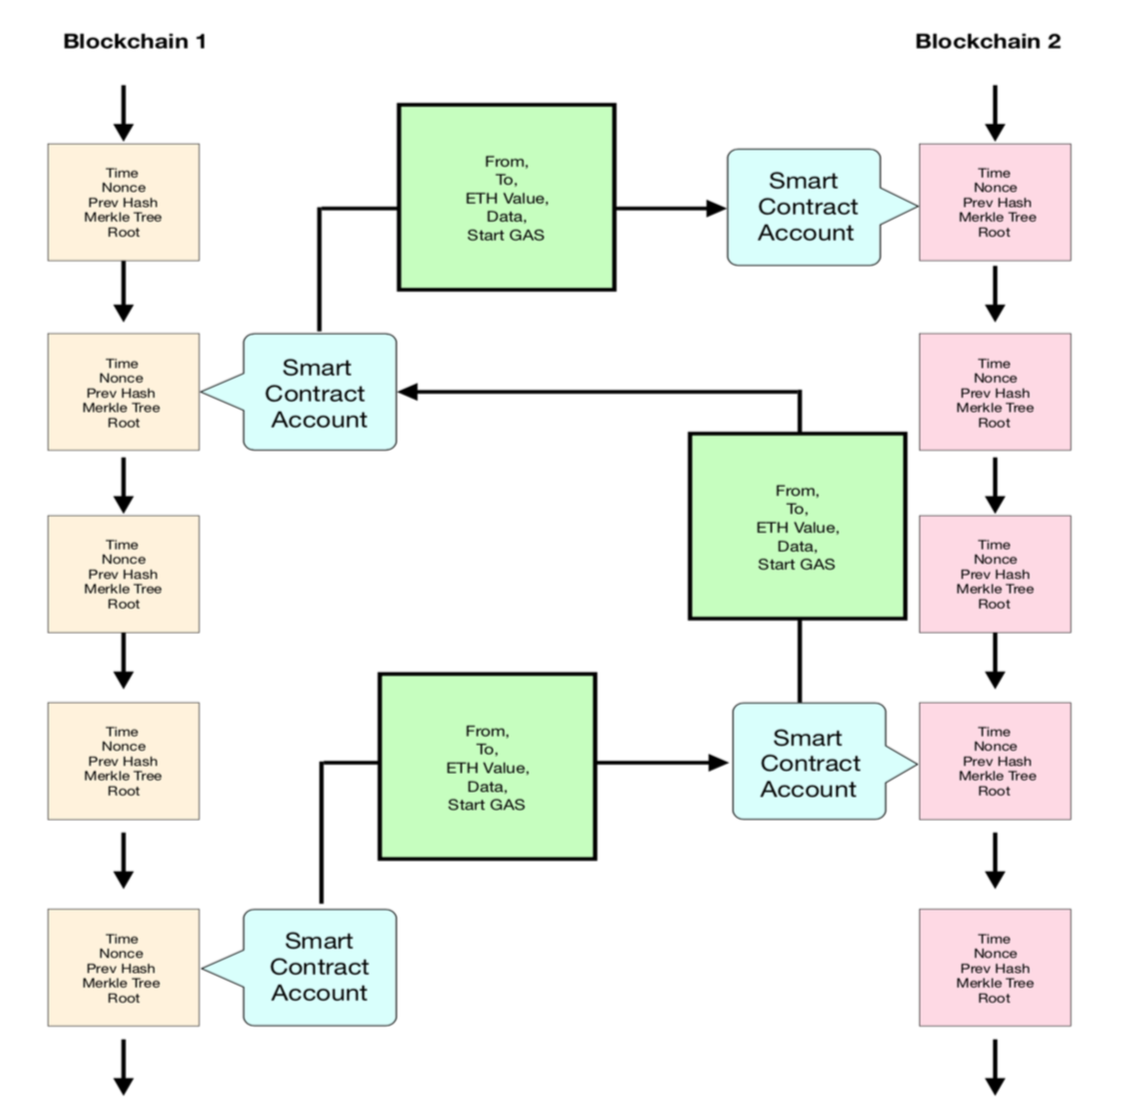
\includegraphics[width=\linewidth]{smart_contract_architecture.png}
  \caption{Smart Contract Architecture}
  \label{fig:A.1}
\end{figure}
\section{Project Timeline}
The thesis project has a very strict timeline and has to be completed within roughly the 15 weeks available in session 2 of 2018. The complete graphical representation of the project timeline has been provided in the GANTT chart attached in appendix I. The first stage of the project which is project planning and literature review has already been completed in this report. The other stages of the project have been described in detail in this section below.
\\
\\
The following provides the detailed timelines of all the tasks that have been identified in the GANTT chart in appendix I:
\begin{enumerate}
    \item \textbf{Project Planning and Literature Review}
    \begin{enumerate}
        \item \textbf{Study Available Research:} In this part of the project, existing research in the field was studied in order to gain in depth knowledge of the field and get a good grasp of the main concepts around blockchain development. This part of the project roughly took 4 weeks to complete, beginning on 26th of February 2018.
        \item \textbf{Find Suitable Background Work:} After studying the available research, work had to be done in order to segregate the research that can be used as a foundation to this particular thesis. All this suitable work has been discussed in the literature review section. This took about 3 weeks to complete.
        \item \textbf{Develop a Timeline:} After the literature review a complete project timeline had to be developed, and all the specific breakdown of tasks and phases had to be identified. This part took roughly about 2 weeks to complete.
        \item \textbf{Write a project plan:} The final part of this project planning stage was actually writing the project plan report for the thesis. This should have taken roughly 4 weeks, however due to exams and unexpected sickness it has taken so long to finish and will be submitted by 2nd July 2018.
    \end{enumerate}
    \item \textbf{App Development and Blockchains Setup}
    \begin{enumerate}
        \item \textbf{Setup a React Native App:} The connectivity suite will have a front-end for
        demonstration purposes. The front-end app will be built using react-native for both
        iOS and Android. This setup will take roughly about 2 weeks.
        \item \textbf{Create two private Ethereum Networks:} The application protocol described in this paper will use these two networks to establish a connectivity suite among them securely. This task is effectively completed, as there are two blockchains already running.
        \item \textbf{Connect the Private networks to the app:} The blockchains will have to be connected to the front-end app in order to demonstrate the connectivity of the two different chains. This task will be done in roughly 1 week.
        \item \textbf{Test the app and blockchain connectivity:} The connectivity between the app and the blockchains has to be tested in order to proceed to the next phases of the project. This will take about a week to test properly.
    \end{enumerate}
    \item \textbf{Develop the Interconnectivity Protocol}
    \begin{enumerate}
        \item \textbf{Build an application to connect the blockchains:} The entire success of the thesis relies on the successful implementation of this part alone. This connectivity protocol is the main feature of the project. Currently, it has been allocated 3 weeks of completion time, however, it might take more, and the timeline will be modified accordingly.
        \item \textbf{Test the Application connectivity:} The connectivity protocol among different blockchains needs to be thoroughly tested for failures and corner cases, and therefore, a week of testing time has been given to this stage.
        \item \textbf{Create a generic protocol from the app:} The paper discusses a protocol for communication among different blockchains and therefore a standard communication protocol that can be applied to multiple blockchains has to be developed, given there is enough time for successful completion. This stage has been allocated a time frame of about 3 weeks.
        \item \textbf{Test the generic protocol:} The generic protocol for smart contract communication will have to be tested on multiple blockchains other than Ethereum for platform independence. The time allocated for this task is about 2 weeks.
    \end{enumerate}
    \item \textbf{Writing the Thesis}
    \begin{enumerate}
        \item \textbf{Write the thesis:} The most important part of the thesis is definitely the thesis. Writing the thesis will take a significant amount of time and therefore a time frame of about 3 weeks has been allocated to this task.
        \item \textbf{Spelling and grammar review:} The thesis will then be checked for any spelling and grammar errors. This is really necessary as it is really easy to go off track with grammar on a thesis of this size. The time allocated for this task is about 4 days.
        \item \textbf{Proof Reading:} The thesis will then need to be proof read for coherence and ease of understanding of the concepts described. This task has been allocated about 5 days.
    \end{enumerate}
    \item \textbf{Peer and Self Review}
    \begin{enumerate}
        \item \textbf{Self-review Thesis:} The thesis will be self-reviewed, and the references will be cross checked before handing it over to the supervisor for suggestions and comments. This task has been given a week for completion.
        \item \textbf{Send for Supervisor Review:} The thesis will then be sent to the supervisor for
        review and comments. Currently, a week’s time has been given to this task, however, this timeline might vary significantly depending on the availability of the supervisor for review. These changes will be appropriately accommodated in the timeline after further consultation with the supervisor.
        \item \textbf{Accommodate changes and suggestions:} The supervisor will definitely have comments and suggestions which will need to be accommodated in the thesis before final submission. This task has been currently allocated about a week, however, the time line will vary depending on the amount of changes suggested by the supervisor. The project timeline will be modified based on the amount work that needs to be done.
        \item \textbf{Final Submission:} The prospective final submission date for the thesis is set on 5th December 2018. However, this date will vary depending on the time taken for supervisor review and the amount of changes that need to be accommodated after the review. Therefore, the final date of submission might vary. Any changes to this date will be communicated with the supervisor in due time.
    \end{enumerate}
\end{enumerate}

\section{Feasibility and Training}
The successful completion of this project relies on a lot of research and innovation. A lot of research has to be accomplished in the area of inter-blockchain communication and networking before a protocol for communication between smart contracts on multiple blockchains can be developed. Some of the successful or partly successful attempts at developing this technology have already been demonstrated in the literature review. Along with the research work available from the literature review, strong grasp of concepts in Networking such UDP, HTTPS, TLS, etc., is required for a successful completion of this thesis. More importantly, concepts in cyber security are extremely important as well. Blockchains heavily use Public Key Infrastructure (PKI); hashing algorithms such as SHA-256, ETH-Hash, etc.; Byzantine Fault Tolerance algorithms and many other mathematically complex algorithms and data structures. Thorough understanding of the above-mentioned algorithms and other consensus algorithms such as proof of work and proof of stake is also extremely necessary.
\\
\\
Ethereum blockchains use a data structure known as Merkle trees in order to store transaction information in the blocks. A thorough understanding of these Merkle tree data structures and Merkle tree headers is really necessary in order to communicate information effectively among blockchains to achieve consensus. Furthermore, a good understanding of the Cryptography and information security concepts taught in COMP343 is also very crucial. All the notes from COMP343 will have to be revised. All the cyber security threats such as DDoS, Man-in-the- middle attack, double spending attack and Sybil fault, etc., will have to be thoroughly reviewed.
\\
\\
The fully spec’d MacBook Pro which is available should be enough for the development of the app and running the Docker containers on Amazon Web Services (AWS) VM instances. However, if there is a possibility of access to a Linux computer or an iMac in one of the computer labs on campus, that would be a very helpful resource towards the project.
\\
\\
The university allows reimbursements of up to \$400 for this thesis project. All of those \$400 will be used towards running Docker containers on AWS VM instances for running the private blockchain nodes. The nodes will be running during testing and prototyping. The instances will be shut down during downtime in order to cut costs. Purchase of any hardware would not be necessary as there is an old iPhone at disposal which can be used for iOS testing purposes and there are multiple emulators available on Android studio for Android testing.

\section{Expected Outcomes and Impact}
The expected outcome of this project is to create a protocol which will allow multiple blockchain networks to send messages among themselves and communicate effectively, using this protocol. This will also include creating a consensus mechanism for all the blocks on the multiple blockchains to validate each other. The blockchains will all be connected to a react- native app which will, in turn, connected to the relay chain. The relay chain will act as a connector blockchain for all the blockchains that are functioning and communicating among themselves. This does seem like a very daunting task for a project that has a time-frame of about 15 weeks. However, if the outcome of the research project is two Ethereum blockchains with multiple smart contracts, all being able to communicate among themselves using the 160- bit addresses, then that would be considered as a positive outcome for the project.
\\
\\
The research project will have three definite outcomes. The first outcome is that the communication protocol among smart contracts on multiple blockchains in possible and successfully implemented. This would be the most ideal outcome and will have the greatest impact in terms of achievement. This could even lead to a fully commercialized technology that will have a massive impact on the entire blockchain industry. The second possible outcome would be that such a communication protocol as described in section 4 of this document is possible, however due to time and resource limitations, such a feat could not be achieved within the time frame of this thesis project. This outcome might not be ideal but leaves room for further development outside the scope of this research thesis and outside the 15 weeks of available time. However, this is still a very positive outcome and further research will be done to accomplish its full effect. The third and the most unwarranted outcome of this research project will be that such connectivity among smart contracts on different blockchains is not possible. This would not be ideal as this would invalidate all the attempts that have been taken so far in this space in order to improve the scalability of all blockchains. This outcome would imply that a completely different approach towards achieving scalability on blockchains has to be taken. Therefore, no matter what the final outcome of this research project is, it is going to revolutionize the way in which the issue of blockchain scalability is being dealt with. The impact of this project is going to be enormous on the entire blockchain ecosystem.
\\
\\
Blockchain technology has the potential to be beneficially applied to numerous different industries. It shows immense ability to disrupt industries like finance, supply chain, energy, software, distributed computing, among many other commercial use cases that are yet to be identified and harnessed. One of the main issues that will stop blockchains from becoming mainstream and going on to disrupt these industries is their ability to scale and handle the millions of transactions which are going to be flooding these blockchains once they are put to effective use. This research addresses the particular issue of scalability facing blockchains. If successful, this project could lead to blockchains becoming effective enough for mainstream use. This will, therefore, lead to complete transition of industries into the age of decentralized computing. It will impact the entire internet and the concept of trust on the internet. The entirely new form of trust on the internet based on mathematical proofs will lead to a new secure, decentralized internet. The impact of this project will be significant on many industries, will disrupt many other and even create a fresh few. The success of this project will be the foundation on which the entire framework of a completely secure and trustless Web 3.0 could be built.
\section{References}
As per the marking rubric, it is mentioned that 4\% of marks for this project plan are contributed from the in-depth review of appropriate peer-reviewed literature. However, due to the uniqueness and novelty of the project, no previous academic or peer-review work is available in this area of blockchain research. All the research and background work has been done by independent third-party organizations and startups. Some of the articles on Medium have also been used for references. The literature review might not be adequate enough due to lack of detailed academic research available. An academic paper even mentions that about 80\% of all academic research in the blockchain space has been done on Bitcoin blockchain alone and only 20\% on other blockchains [15]. Therefore, marker’s attention towards this fact is being requested and marking this particular criterion for the project plan is requested to be done considerately.
\begin{description}
\item[[1]]M. Zago, ``Why the Web 3.0 Matters and you should know about it",
CoinDesk Newsroom.mastercard.com
Medium, 2018.[Online]. Available:https://medium.com/@matt\\eozago/why-the-web-3-0-matters-and-you-should-know-about-it-a5851d63c949. [Accessed: 09- Jun- 2018].
\item[[2]]A. Hertig, ``How Will Ethereum Scale? - CoinDesk", CoinDesk
, 2018. [Online]. Available:
 https://www.coindesk.com/information/will-ethereum-scale/. [Accessed: 06- Jun- 2018].
\item[[3]``Bitcoin and Ethereum vs Visa and PayPal – Transactions per second - Altcoin
  Today",
Altcoin Today
, 2018. [Online]. Available: https://altcointoday.com/bitcoin-ethereum-
 vs-visa-paypal-transactions-per-second/. [Accessed: 11- Jun- 2018].
\item[[4]]``The MasterCard Network Advantage", Newsroom.mastercard.com
, 2018. [Online].
 Available: https://newsroom.mastercard.com/wp-content/uploads/2011/09/Master\\Card-
 Network-Advantage.pdf. [Accessed: 11- Jun- 2018].
\item[[5]] ``State of the ÐApps — What's a ÐApp",
https://www.stateofthedapps.com/whats-a-dapp. [Accessed: 13- Jun- 2018].
\item[[6]]  ``Ethereum/wiki", Github, 2014, [Online]. https://github.com/ethereum/wiki/wiki/White-Paper. [Accessed: 14- Jun- 2018].
\item[[7]] ``BTC Relay",Btcrelay.org, 2016. [Online]. Available: http://btcrelay.org. [Accessed: 18-
Jun- 2018].
\item[[8]]``Frequently Asked Questions — BTC Relay 1.0 documentation", https://btc-relay.readthedocs.io\\/en/latest/
 2018. [Online]. Available: http://btc-relay.readthedocs.io/en/latest/frequently-asked-
 questions.html. [Accessed: 15- Jun- 2018].
\item[[9]]L. Luu, ``PeaceRelay: Connecting the many Ethereum Blockchains", Medium
, 2017.
 [Online]. Available: https://medium.com/@loiluu/peacerelay-connecting-the-many-ethereum-
 blockchains-22605c300ad3. [Accessed: 19- Jun- 2018].
\item[[10]] J. Kwon and E. Buchman, ``cosmos/cosmos",
GitHub, 2018. [Online]. Available:
 https://github.com/cosmos/cosmos/blob/master/WHITEPAPER.md\#inter-blockchain-
 communication-ibc. [Accessed: 24- Jun- 2018].
\item[[11]]G. Wood, ``Polkadot Light-paper", Polkadot.network
, 2018. [Online]. Available:
 https://polkadot.network/Polkadot-lightpaper.pdf. [Accessed: 23- Jun- 2018].
\item[[12]]G. Wood, ``POLKADOT: VISION FOR A HETEROGENEOUS MULTI-CHAIN
  FRAMEWORK",
Polkadot.\\network
, 2016. [Online]. Available:
 https://polkadot.network/PolkaDotPaper.pdf. [Accessed: 18- Jun- 2018].
\item[[13]]``Interledger Protocol V4 (ILPv4) | Interledger",
Available: https://interledger.org/\\rfcs/0027-interledger-protocol-4/. [Accessed: 29- Jun- 2018].
Interledger.org
Interledger.org
Btc-relay.readthedocs.io,
Medium
, 2018. [Online].
\item[[14]] ``STREAM
- A
Multiplexed
Money and Data Transport for ILP |
PLOS ONE
  Interledger", interledger.org
, 2018. [Online]. Available: https://interledger.org/rfcs\\/0029-
 stream/\#33-multiplexed-streams. [Accessed: 29- Jun- 2018
\item[[15]] J. Yli-Huumo, D. Ko, S. Choi, S. Park and K. Smolander, "Where Is Current Research on
  Blockchain Technology? —A Systematic Review", PLOS ONE
, vol. 11, no. 10, p. e0163477,
 


\end{description}
\chapter{Ethereum WhitePaper}
\section{Overview}
here is the Overview of appendix B ...
\section{}
here is the content of this section ...

\chapter{genesis.json for Tendermint}
\lstset{%
   breaklines=true
}
\begin{lstlisting}
{
  "genesis_time": "2016-02-05T06:02:31.526Z",
  "chain_id": "chain-tTH4mi",
  "validators": [
    {
      "pub_key": [
        1,
        "9BC5112CB9614D91CE423FA8744885126CD9D08D9FC9D1F42E552D662BAA411E"
      ],
      "power": 1,
      "name": "mach1"
    },
    {
      "pub_key": [
        1,
        "F46A5543D51F31660D9F59653B4F96061A740FF7433E0DC1ECBC30BE8494DE06"
      ],
      "power": 1,
      "name": "mach2"
    },
    {
      "pub_key": [
        1,
        "0E7B423C1635FD07C0FC3603B736D5D27953C1C6CA865BB9392CD79DE1A682BB"
      ],
      "power": 1,
      "name": "mach3"
    },
    {
      "pub_key": [
        1,
        "4F49237B9A32EB50682EDD83C48CE9CDB1D02A7CFDADCFF6EC8C1FAADB358879"
      ],
      "power": 1,
      "name": "mach4"
    }
  ],
  "app_hash": "15005165891224E721CB664D15CB972240F5703F",
  "app_state": {
    {"account": "Bob", "coins": 5000}
  }
}

\end{lstlisting}
\chapter{genesis.json for Ethereum}
\begin{lstlisting}
{
    "nonce": "0xdeadbeefdeadbeef",
    "timestamp": "0x0",
    "parentHash": "0x0000000000000000000000000000000000000000000000000000000000000000",
    "extraData": "0x0",
    "gasLimit": "0x8000000",
    "difficulty": "0x400",
    "mixhash": "0x0000000000000000000000000000000000000000000000000000000000000000",
    "coinbase": "0x3333333333333333333333333333333333333333",
    "alloc": {
    }
}
\end{lstlisting}
\bibliographystyle{acm}
\bibliography{my_reference}

\end{document}
